\documentclass[11pt,a4paper, titlepage]{article}

\usepackage[utf8]{inputenc}
\usepackage{amssymb}
\usepackage{graphicx,wrapfig}
\usepackage{float}
\usepackage[export]{adjustbox}
\usepackage{array}
\usepackage{comment}
\usepackage{tabularx,longtable}
\usepackage{amsmath}
\usepackage{amsfonts}
\usepackage{subcaption}
\usepackage[toc,page]{appendix}

\renewcommand{\baselinestretch}{1.5}

\usepackage[width=16.00cm, left=2.50cm, top=2.5cm, bottom=2.5cm]{geometry}

\title{ARPA: Autonomous Robotic Pointer Arm}
\author{Helgerud, Erlend \and Håland, André}

\begin{document}
	\setlength\parindent{0pt}
	\setlength\parskip{10pt}
	\headheight
	\setlength{15pt}{}
	\footskip
	\setlength{33pt}{}
	\setcounter{secnumdepth}{4}
	\maketitle
	
\begin{abstract}
This report is written as part of a project in the course DFMS3200 - Simulation and Modelling at the University College of South-Eastern Norway. The background for the project is the idea of automation in industrial production lines in order to minimize costs and increase productivity. The solution proposed is an autonomous 5DOF robotic manipulator that perform actions based on a live video feed. The main focus of the project is to serve as a introductory case-study in robotic manipulation and control, and therein the usage of selected tools. The project is split in two, virtual simulation and physical representation. For controlling both the virtual and physical representation, the project utilizes ROS Kinetic (Robotic Operating System) in Ubuntu 16.04 with the majority of code written in C++. The physical robot is powered by 12 AA batteries together with two Arduino MEGA2560's. The vision system is based in Python 2.6 and OpenCV2. In order to provide the virtual representation the project incorporates Gazebo together with needed models written in URDF/Xacro and configurations written in YAML. Kinematics are handled in Matlab's Robotics System Toolbox. As a final demonstration, the separate components of the project will be run with a 1:1 relationship between the virtual and physical representations, integrating all components of the project.
\end{abstract}
	
	\tableofcontents
	\newpage

\section{Introduction}
As a result of the high average of salaries in Norway a lot of the processing of food is outsourced to countries with a lower average salary \cite{berge2015}. An example is the outsourcing of processing of Norwegian salmon to Poland, which has a lower hourly rate of work by 13.5\% compared to Norway. A direct consequence of the difference is that companies like Marine Harvest export roughly processed salmon to Poland, and import fine processed salmon back to Norway \cite{digre2014}. To be able to preserve the processing of fish in Norway, there is a demand for a system that can remove defects such as blood and/or melanin defects from the surface of fish fillets.

Using the previous paragraph as the background, the motivation for this project is to conduct case-study in robotic manipulation and control in order to be familiarized with possible tools and technologies used in robotics.

The project itself has served as an introduction to robot technology, thus, a big part of the project has been the learning of the different technologies which will be discussed in detail later in the report.

\subsection{Goals}
The following goals were set for the project:
\begin{itemize}
\item Gain knowledge in Robotics Operating System
\item Develop a fully functioning prototype
	\begin{itemize}
	\item 1:1 relationship between physical and virtual model
	\item Actions based on object-detection
	\item Develop own kinematic model	
	\end{itemize}
	
\end{itemize}

\subsection{Contributions}
The project aims to contribute an environment consisting of a physical 5DOF robotic manipulator with a 1:1 relationship to a virtual simulation which can be used for rapid prototyping and testing. The system has incorporated a detection system to automate the process of finding markers. In addition, the delivered report and GitHub repository should serve as a contribution to student inheriting the project at a later stage.

The physical robot is powered by two Arduino Mega2560's and 12 AA batteries. One of the Arduinos functions as the controller for the physical robot, while the other one serves solely as a power supply to a servo motor.

\subsection{Tools}
The tools used in ARPA, both in terms of hardware and software are presented in the following sections.

\subsubsection{Hardware}

Table \ref{hardware} shows a list of the hardware components used in ARPA. The robotic manipulator is not listed, nor are bare necessities such as wiring etc.

	\begin{center}           
    \begin{longtable}{| l | c | c |}
              \hline
%Utvid ved å kopiere: xx.xx.2018 & IDXX & Oppdatering \\  \hline            
\multicolumn{3}{|c|}{\textbf{Hardware}} \\ \hline \endhead
\textbf{Component} & \textbf{Quantity} & \textbf{Usage} \\ \hline             
              \textbf{Hitec HS-475HB Servo} &  1 & 4th joint \\ \hline
              
              \textbf{Sanwa Hyper ERG-VZ Servo} &  2 & 2nd and 3rd joint \\ \hline
             
              \textbf{Savox Digital SC0252MG Servo} & 1 & 1st joint \\ \hline
              
              \textbf{Parallax Standard Servo} & 1 & 5th joint \\ \hline
              
              \textbf{Creative Labs Webcamera} & 1 & Detection system  \\  \hline
              
              \textbf{Arduino MEGA2560} & 2 & Control and power  \\ \hline
              
              \textbf{4x AA Battery Pack} & 3 & Power   \\  \hline

\caption{Hardware used in ARPA}
\label{hardware}                                       
\end{longtable}
\end{center}



\subsubsection{Software dependencies}

Table \ref{software} shows a list of the software dependencies for running ARPA.

\newpage

	\begin{center}           
    \begin{longtable}{| l | l |}
              \hline
%Utvid ved å kopiere: xx.xx.2018 & IDXX & Oppdatering \\  \hline            
\multicolumn{2}{|c|}{\textbf{Software}} \\ \hline \endhead
\textbf{Software} & \textbf{Usage} \\ \hline             
              \textbf{Ubuntu 16.04 LTS} & Operating System \\ \hline
              
              \textbf{ROS Kinetic} & Framework for robot software \\ \hline
              
              \textbf{Gazebo} & Simulation environment \\  \hline
             
              \textbf{rosserial\_arduino} & Include Arduino into ROS node network \\ \hline
              
              \textbf{MATLAB: Robotics System Toolbox} & MATLAB add-on providing different robotic software \\ \hline
              
              \textbf{OpenCV2} & Computer vision library used with Python \\  \hline

\caption{Software dependencies}
\label{software}                                       
\end{longtable}
\end{center}     

\subsection{Content}
In addition to the introduction, this report consists of \textbf{\ref{relwork}: Related works}, \textbf{\ref{description}: System description}, \textbf{\ref{simex}: Simulations and experiments} and \textbf{\ref{discussion}: Discussion}

\section{Related works}
\label{relwork}
Robotics is a wide field, and many projects have been conducted. This ection will compare some related work to this project.

\subsection{Robot arm control with Arduino}
The work in this report is conducted by Abdellatif Baba. Need for help systems in everyday life, and the evolution of autonomous systems is the background for the project. To solve this, Baba is looking to design a robot arm which takes a piece of material and moves it to a desired position. The movement should be recorded, and the arm should continue to do the action until the user tells it to stop \cite{baba2017}. Table \ref{comp-table1} shows a comparison of ARPA and Robot arm control with Arduino (RACWA)

\begin{center}           
    \begin{longtable}{| p{8cm} | p{8cm} |}
              \hline
                       
\multicolumn{2}{|c|}{\textbf{Comparison}} \\ \hline \endhead
\textbf{ARPA} & \textbf{RACWA}  \\ \hline             
               Background in automation & Background in automation  \\ \hline
               Uses Arduino Mega2560 & Uses Arduino Nano  \\ \hline
               Uses five servo motors & Uses five servo motors \\ \hline
               Wired communication between PC and Arduino  & Communication through Bluetooth on Arduino with Android application \\ \hline
               Uses ROS & Does not use ROS \\ \hline
               Model visualized in simulation environment & No visual model \\ \hline
               
\caption{Comparison of ARPA and RACWA}
\label{comp-table1}                                       
\end{longtable}
\end{center}


\subsection{Anthropomorphic Robotic Manipulator}
The work in this report is conducted by Jeffry Walker, Joshua Beverly, Christopher Cook and Migueal de Rojas. The goal of the project was to design a 5 DOF Anthropomorphic Geometry Manipulator (APGM) with a gripper as end-effector. The end-effector should be able to lift a cube with lengths of 5cm and mass of 0.34kg and place it between two predetermined spatial coordinates \cite{walker2012}. Table \ref{comp-table2} lists some of the differences and similarities between ARPA and Anthropomorphic Robotic Manipulator (ARM).

\begin{center}           
    \begin{longtable}{| p{8cm} | p{8cm} |}
              \hline
                       
\multicolumn{2}{|c|}{\textbf{Comparison}} \\ \hline \endhead
\textbf{ARPA} & \textbf{ARM}  \\ \hline             
                Five DOF & Five DOF  \\ \hline
                A simple poker as end-effector & Parallel opening gripper as end-effector  \\ \hline
               Moves to camera detected marker & Moves to predetermined points and picks up object and moves it to predetermined spot  \\ \hline
                Uses five servo motors  & Uses five DC motors with optical encoders used to PID regulate  \\ \hline
                Uses Arduino Mega & Uses Arduino Mega   \\ \hline
               
\caption{Comparison of ARPA and ARM}
\label{comp-table2}                                       
\end{longtable}
\end{center}






\section{System description}
\label{description}
	

\subsection{Architecture}
The idea of ARPA is to have a 1:1 relationship between a physical robotic arm, and a model in Gazebo. This means that the model in Gazebo should contain (as good as) the same measurements as the physical robot. They will also receive the same control signals leading to synchronized movement. Figure \ref{fig:architecture} show this relationship between the real world and the simulated world.
	
	\begin{figure}[H]
		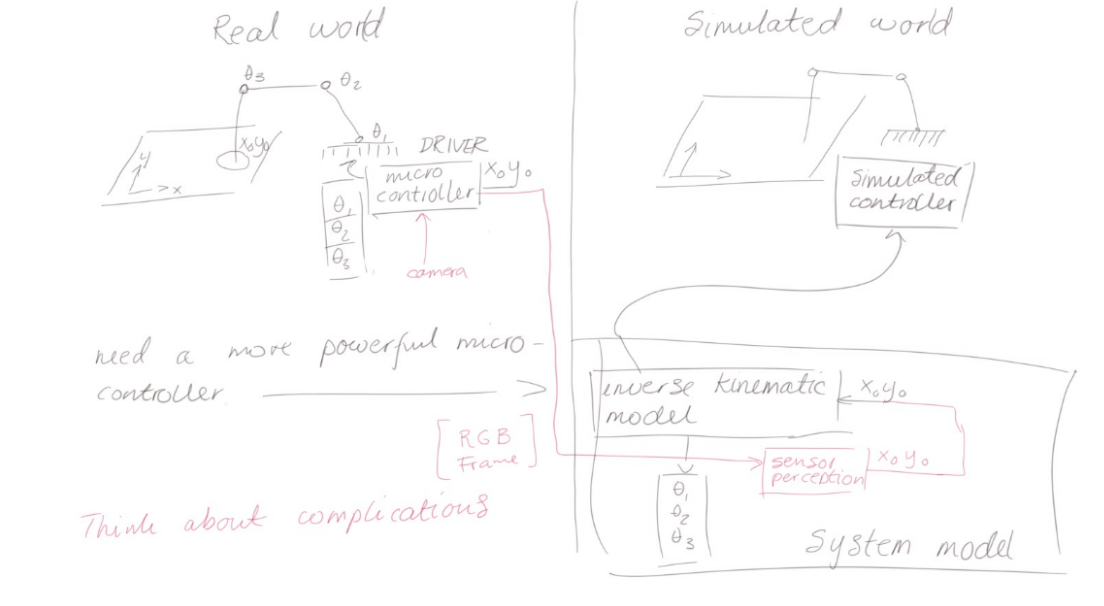
\includegraphics[width=\linewidth]{../Diagrams/Architecture.png}
		\caption{System architecture}
		\label{fig:architecture}
	\end{figure}
	
	ARPA is divided into nodes. These nodes each has its own tasks and communicate with each other on different topics to exchange information. Figure \ref{fig:nodegraph} shows the nodes of ARPA, and the topics they communicate on. A circle represents a node, whilst a rectangle represents a topic. The controller node is the center of all actions. It handles the interface between the camera, MATLAB, the physical robotic arm and the model in gazebo. The camera node  sends a Cartesian point in space to the controller. The MATLAB node handles inverse kinematics. It receives Cartesian coordinates from the controller, and sends back five joint angles. The 5DOF Robot node controls the physical robotic arm by writing received angles to the servo motors. The Gazebo node listens to the same topics as 5DOF Robot, and will simulate a robotic model with a 1:1 relationship with the physical arm.
	
	\begin{figure}[H]
		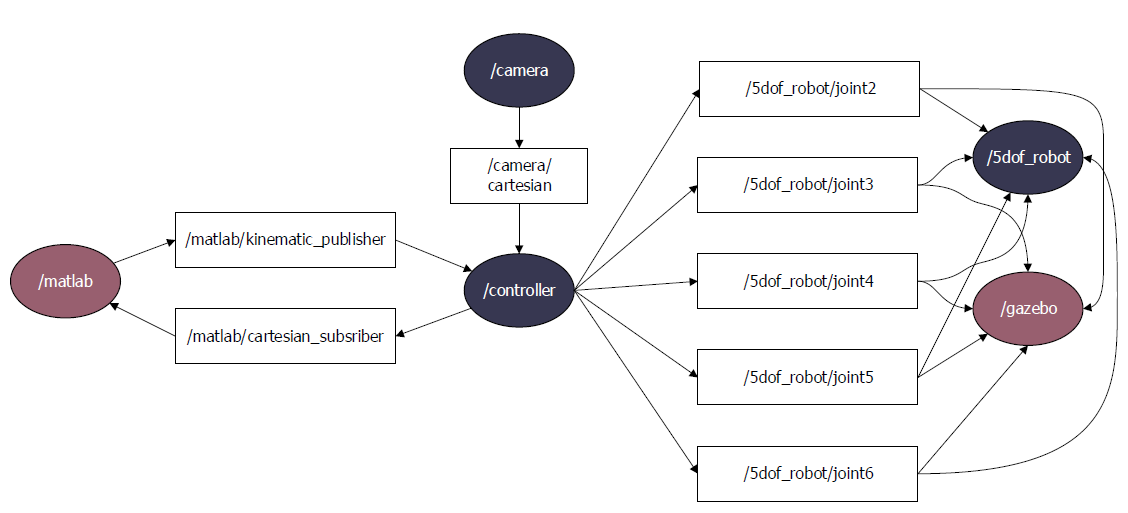
\includegraphics[width=\linewidth]{../Diagrams/NodeGraph-v1.png}
		\caption{Node graph}
		\label{fig:nodegraph}
	\end{figure}
	
As described in \textit{\ref{invkin} Inverse kinematics}, we had some challenges with finding the inverse kinematics and have to depend on the Robotics System Toolbox from MATLAB. When running MATLAB as a ROS node, we discovered that it ran quite slowly together with Gazebo. For this reason, we decided to run the ROS network over two computers to separate computing power. This is done by setting a couple of environmental variables in every terminal that uses ROS. Two shell scripts were made for this, and can be sourced to achieve the distributed ROS network. The different colored nodes in figure \ref{fig:nodegraph} represents which computer the node runs on.

	
The nodes previously described is made by ROS packages. Figure \ref{fig:dir-list} shows the packages used in ARPA. The following subsections will describe each package, including why and how they are implemented.

	\begin{figure}[H]
		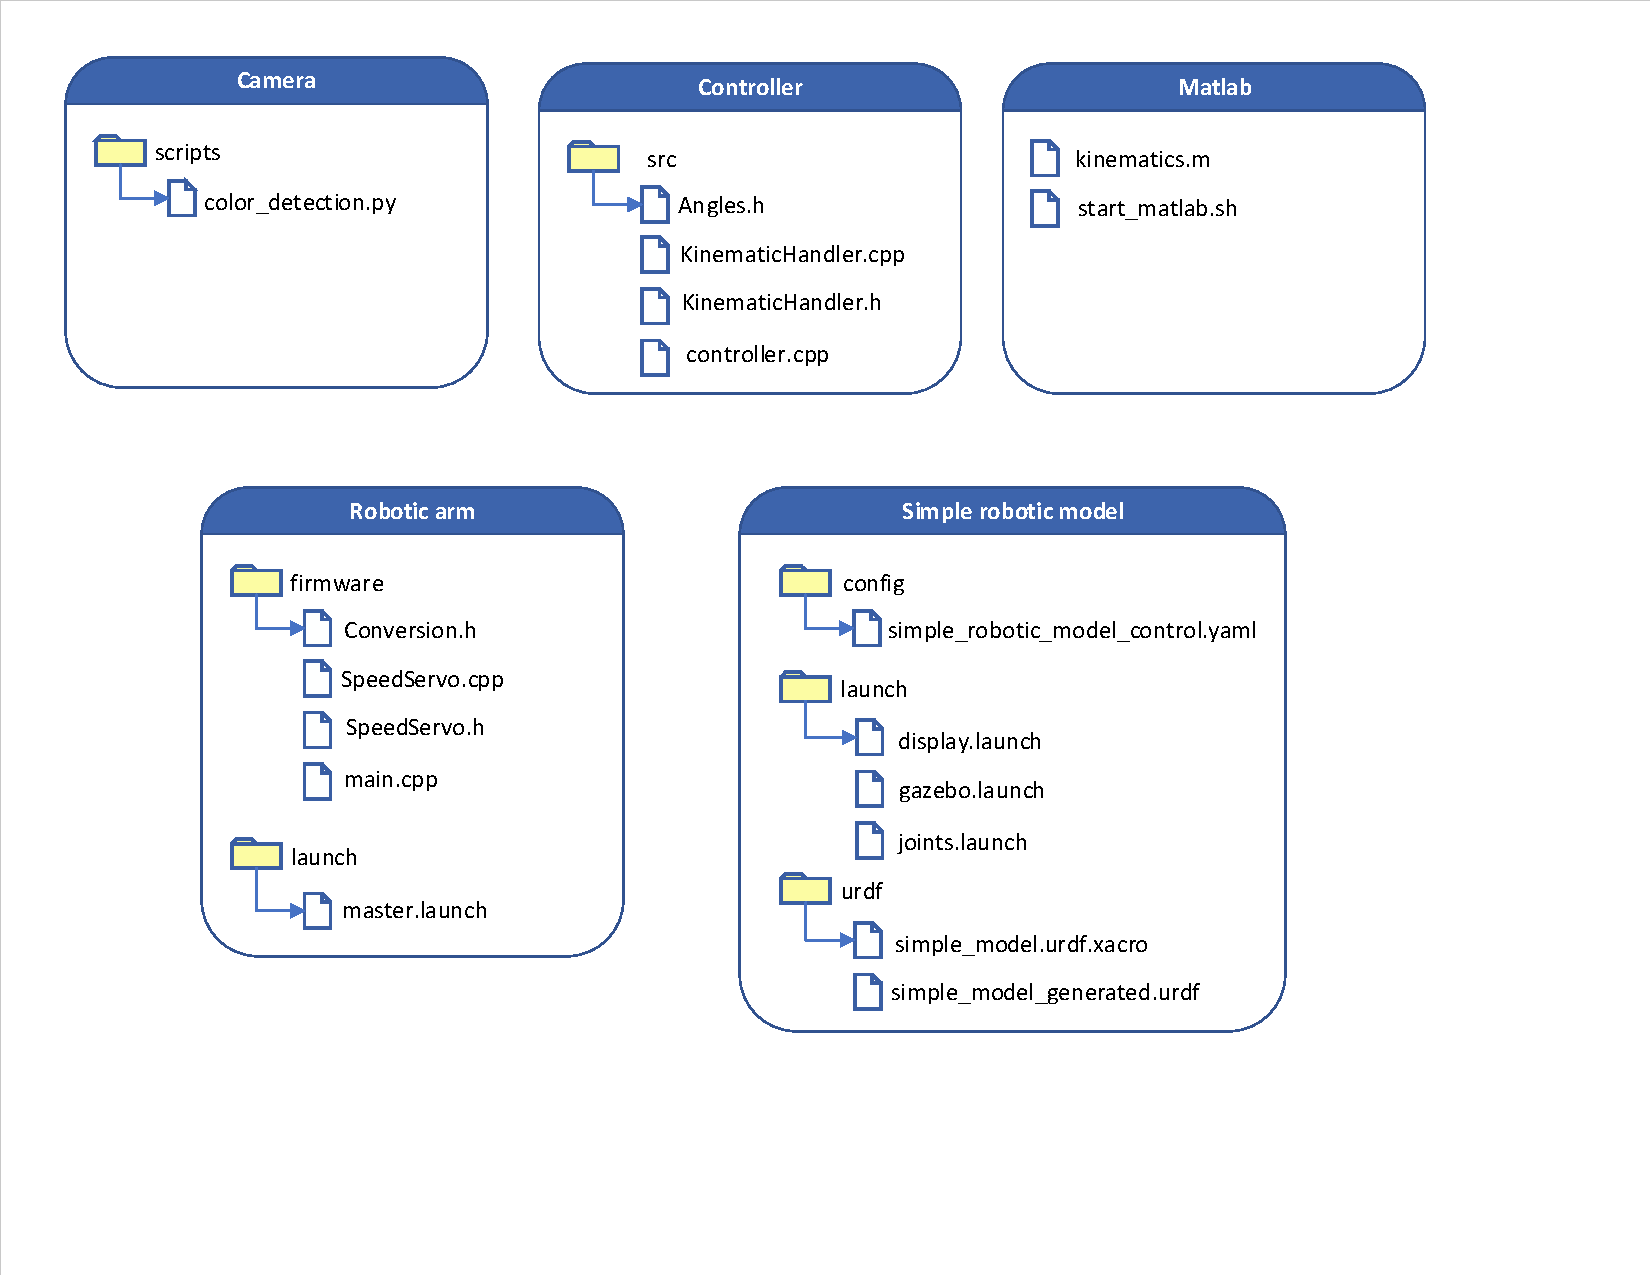
\includegraphics[width=\linewidth]{../Diagrams/Packages.png}
		\caption{Packages}
		\label{fig:dir-list}
	\end{figure}
	
	
\subsubsection{Camera}
The camera package contains the python-script that is responsible for handling object detection in ARPA. By placing red markers in the physical coordinate system of ARPA, the user will be able to track the markers with the live video feed from OpenCV. The script will after calibration continuously map received coordinates from the OpenCV coordinate frame to coordinates corresponding to the physical coordinate frame on the rig. The calibration and usage during runtime will be elaborated in finer detail in \textit{\ref{calibratecam} Calibration of camera}.

The color-detection is done by applying a red mask in the HSV-colorspace on each frame from the live video. By finding the contours of the image the marker can be detected and the script further finds the center of the detected point. The script is incorporated in the ROS environment as a node that publishes the mapped cartesian x and y coordinates of a desired point. The script can be extended to detect more colors by adding additional

\subsubsection{Controller}
The controller package handles the interface between the other nodes. First of all, it receives all the coordinates from the camera node, but will only publish them to MATLAB if the \textit{ready.sh} script has been run. Optionally, a message containing a  "1" (boolean true) can be published on the\textit{/camera\_ready} topic. After the controller has published the coordinates to MATLAB, it will receive a response in the form of five joint angles. These joint angles are further sent to their respective topics. Immediately after the angles are published, the controller sleeps for five seconds. During these five seconds, the robotic arm will have time to go to the given coordinates. After sleeping, the controller will start a function that sets the arm to a upright position, hereby referred to as the start position of the arm. It does so by rotating the top servos the opposite direction of the bottom servos, before it rotates the bottom servos. This is done because the torque of the bottom servos are to big to directly set all joints to start position. After approximately using three seconds to set the arm to start position, the controller is ready to get a new ready signal from the user.

\subsubsection{Matlab}
The matlab package is responsible for solving the inverse kinematics for ARPA. The matlab script contained in kinematics.m is integrated in the ROS environment through the Robotics System Toolbox, allowing Matlab to act as a standalone node in the graph. The script subscribes to the cartesian\_subscriber which receives messages from the camera. When messages are received, the callback is initialized which derives the inverse kinematics with a numerical approach.

The inverse kinematics solver is based on a URDF model of the robot, which means it can return inverse kinematics for any given 5DOF robotic manipulator. The script publishes the derived values of $\theta_n$ in the form of a Float64MultiArray to the kinematic\_publisher, which in turn is subscribed to by the controller.

\subsubsection{Robotic arm}
The robotic arm package contains the software running on the Arduino to control the servo motors. The main task of this node is to receive joint angles from the controller, and set the servo motors to the correct position. To control the servo motors, the native servo library provided by Arduino is used.

Writing a joint angle directly to the servo motors makes the servos rotate at maximum speed. To slow down the angular velocity of the motors, the robotic arm package implements a class which slowly increments the write-value sent to the servos. This speed of the servos can then be changed by adjusting how often the write value should be incremented.

This package also contains the launch file running the controller- and camera node in addition to the robotic arm node. Refer to \textit{\ref{startup} Starting program} for how to use the launch file.
	

\subsubsection{Simple robotic model}
The simple robotic model package contains the URDF/Xacro used to model the virtual representation of the robot. It contains one Xacro file, which is programmed, and the generated URDF file that is used in Gazebo. The launch files are located in the launch directory, where joints.launch is the master launch file. This file includes the generated URDF model aswell as it includes the gazebo.launch file. The joints.launch will also launch the MATLAB node. The YAML file simple\_robotic\_model.control in the config directory contains the configurations for the joint\_state\_controller, which handles position control of the joints of ARPA.
	
\subsection{Information flow}
The flow of information in ARPA starts when the user sends a ready signal to the controller node. This signals that the controller will accept a Cartesian coordinate from the camera. This coordinate  further sent to MATLAB for processing. MATLAB returns five joints angles to the controller. These are the angles used to control both the physical arm and the Gazebo model. Hence, the controller publishes them to their respective topics, where they are picked up by both the Gazebo node and the 5DOF Robot node. After the control node has sent the joint angles, it waits for 5 seconds before it sends a new set of joint angles used to set the physical and simulated arm back to starting position. This process can be repeated by sending a new ready signal. Figure \ref{fig:seq-diagram} shows the flow of information in the form of a UML Sequence diagram.
	
	
	\begin{figure}[H]
		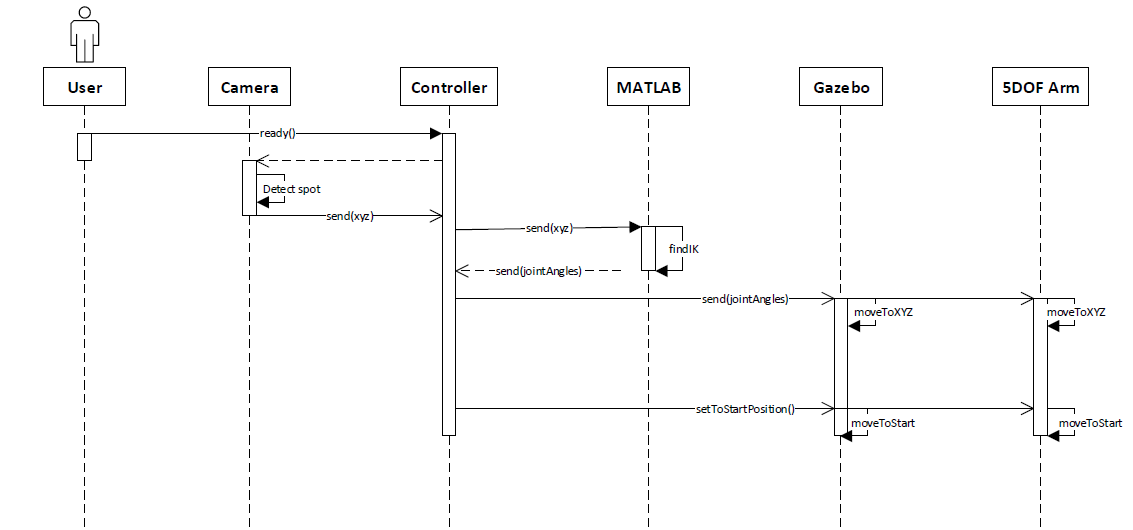
\includegraphics[width=\linewidth]{../Diagrams/SequenceDiagram-v1.png}
		\caption{UML Sequence diagram}
		\label{fig:seq-diagram}
	\end{figure}
	
	\subsection{Use case}
	The different actors involved in ARPA and their main use cases are shown in the form a a UML use case diagram in figure \ref{fig:use-case}.
	
	\begin{figure}[H]
		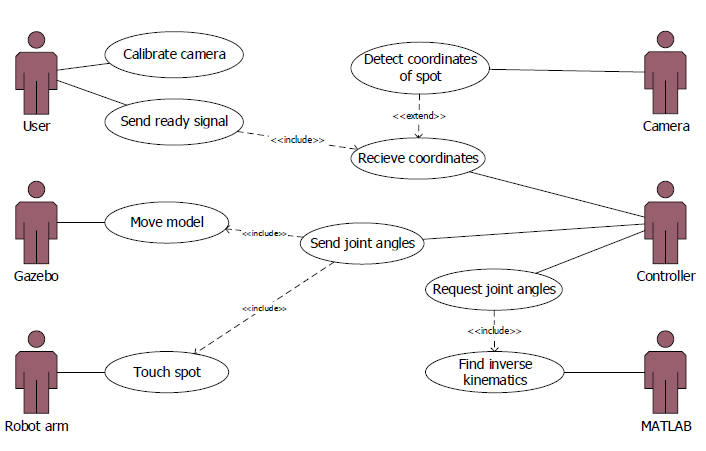
\includegraphics[width=\linewidth]{../Diagrams/UseCase.png}
		\caption{UML Use case}
		\label{fig:use-case}
	\end{figure}
		
	
	\subsection{Starting program}
	\label{startup}
	
	When running ARPA over two computers, one of them must be chosen to run as the ROS master. The selected master computer must source the master.sh script in every terminal used for running ROS commands. Next, the slave.sh script must be modified to contain the IP-address of the master computer. The address can be read from the output of the master.sh script. When the slave script is modified to contain the correct address, it must be sourced in all terminals on the slave computer that runs any ROS commands.
	
	Next up is to launch all ROS nodes. First of all, the setup.bash script in the devel directory of the catkin workspace must be sourced. When this is done on the master computer, the Arduino controlling the servos of the robotic arm must be connected to the computer. When it is connected, the command \textit{roslaunch robotic\_arm master.launch} can be run. Note that the launch file is configured to setup the ROS node on /dev/ttyACM0. This means that either the Arduino running the code must be connected before the Arduino used for power supply (see \textit{\ref{power} Power Supply}), or the launch file must be modified to contain the correct device parameter. The roslaunch command starts the camera, controller and the 5DOF robot node. 
	
\subsubsection{Calibration of camera}
\label{calibratecam}
The detection system used in ARPA is based in Python and the OpenCV library, and can be used together with an internal or external camera. The python script is in the beginning made so that a user has to go through a calibration phase to ensure mapping from the OpenCV coordinate frame to the coordinate frame of the physical rig.

Before running \textit{roslaunch robotic\_arm master.launch} there should be a red marker placed in ARPA's origo. The x-axis on the physical rig should also be parallel with the bottom border of the OpenCV window frame. The camera will during the first five seconds self-calibrate for lighting and focus, before masking the picture to find the red marker representing origo. After capturing 50 frames there is a five second pause in which the user will have to move the marker from origo to x-max, after an additional 50 frames the same will be repeated for y. When the script has defined all needed points of the coordinate frame, the values from the OpenCV frame is mapped to the lengths of the physical coordinate frame defined in the script. This method ensures that the same calibration method can be used independent of the cameras height above the rig, as long as origo, x-max and y-max is in the camera-frame.
	
	As with the master computer, the slave must also source the setup.bash script in the devel directory of the catkin workspace. When this is done, the command \textit{roslaunch simple\_robotic\_model joints.launch} can be run. This starts both the Gazebo and MATLAB node.
	
	\subsection{User interface}

	The user interface of ARPA is split into two: one on the master computer and one on the slave computer. Figure \ref{fig:ui-master} shows the user interface of the master. The window to the left is a live feed of the camera. It shows the user the detection of a red dot, i.e. where ARPA will move when given a ready signal. The window to the right allows the user to send this ready signal. When the ready.sh script is executed, the controller node will accept the next incoming coordinates and execute all necessary communications and actions for both the physical arm and the Gazebo model to move.
	
	\begin{figure}[H]
		\centering
		\includegraphics[width=0.95\linewidth]{../Diagrams/UI-master.png}
		\caption{User interface: Master}
		\label{fig:ui-master}
	\end{figure}
	
	Figure \ref{fig:ui-slave} shows the user interface of the slave. Gazebo is launched as described in \textit{\ref{startup} Starting program}, but the rqt window on the left is not included as a part of the launch file. The user can choose to start rqt from a new terming through the \textit{rqt} command. The preferred setup for this project was to have rqt run the console plugin to show all the ROS messages in a GUI.
	
	\begin{figure}[H]
		\centering
		\includegraphics[width=0.95\linewidth]{../Diagrams/UI-slave.png}
		\caption{User interface: Slave}
		\label{fig:ui-slave}
	\end{figure}
	
	\subsection{Hardware}
	During the project we had to make some adjustments to parts of the hardware related to the robotic arm. This section will go explain which adjustments has been made, and why.
	\subsubsection{Rig}
	When we were handed the robotic arm at the beginning of the course, we did some testing of it. First of all, we discovered that it both had some loose screws, and were also missing some. This lead us to spending some time on making the arm more rigid and secure. Figure \ref{fig:early-rig} shows this stage of the project.
	
	\begin{figure}[H]
		\centering
		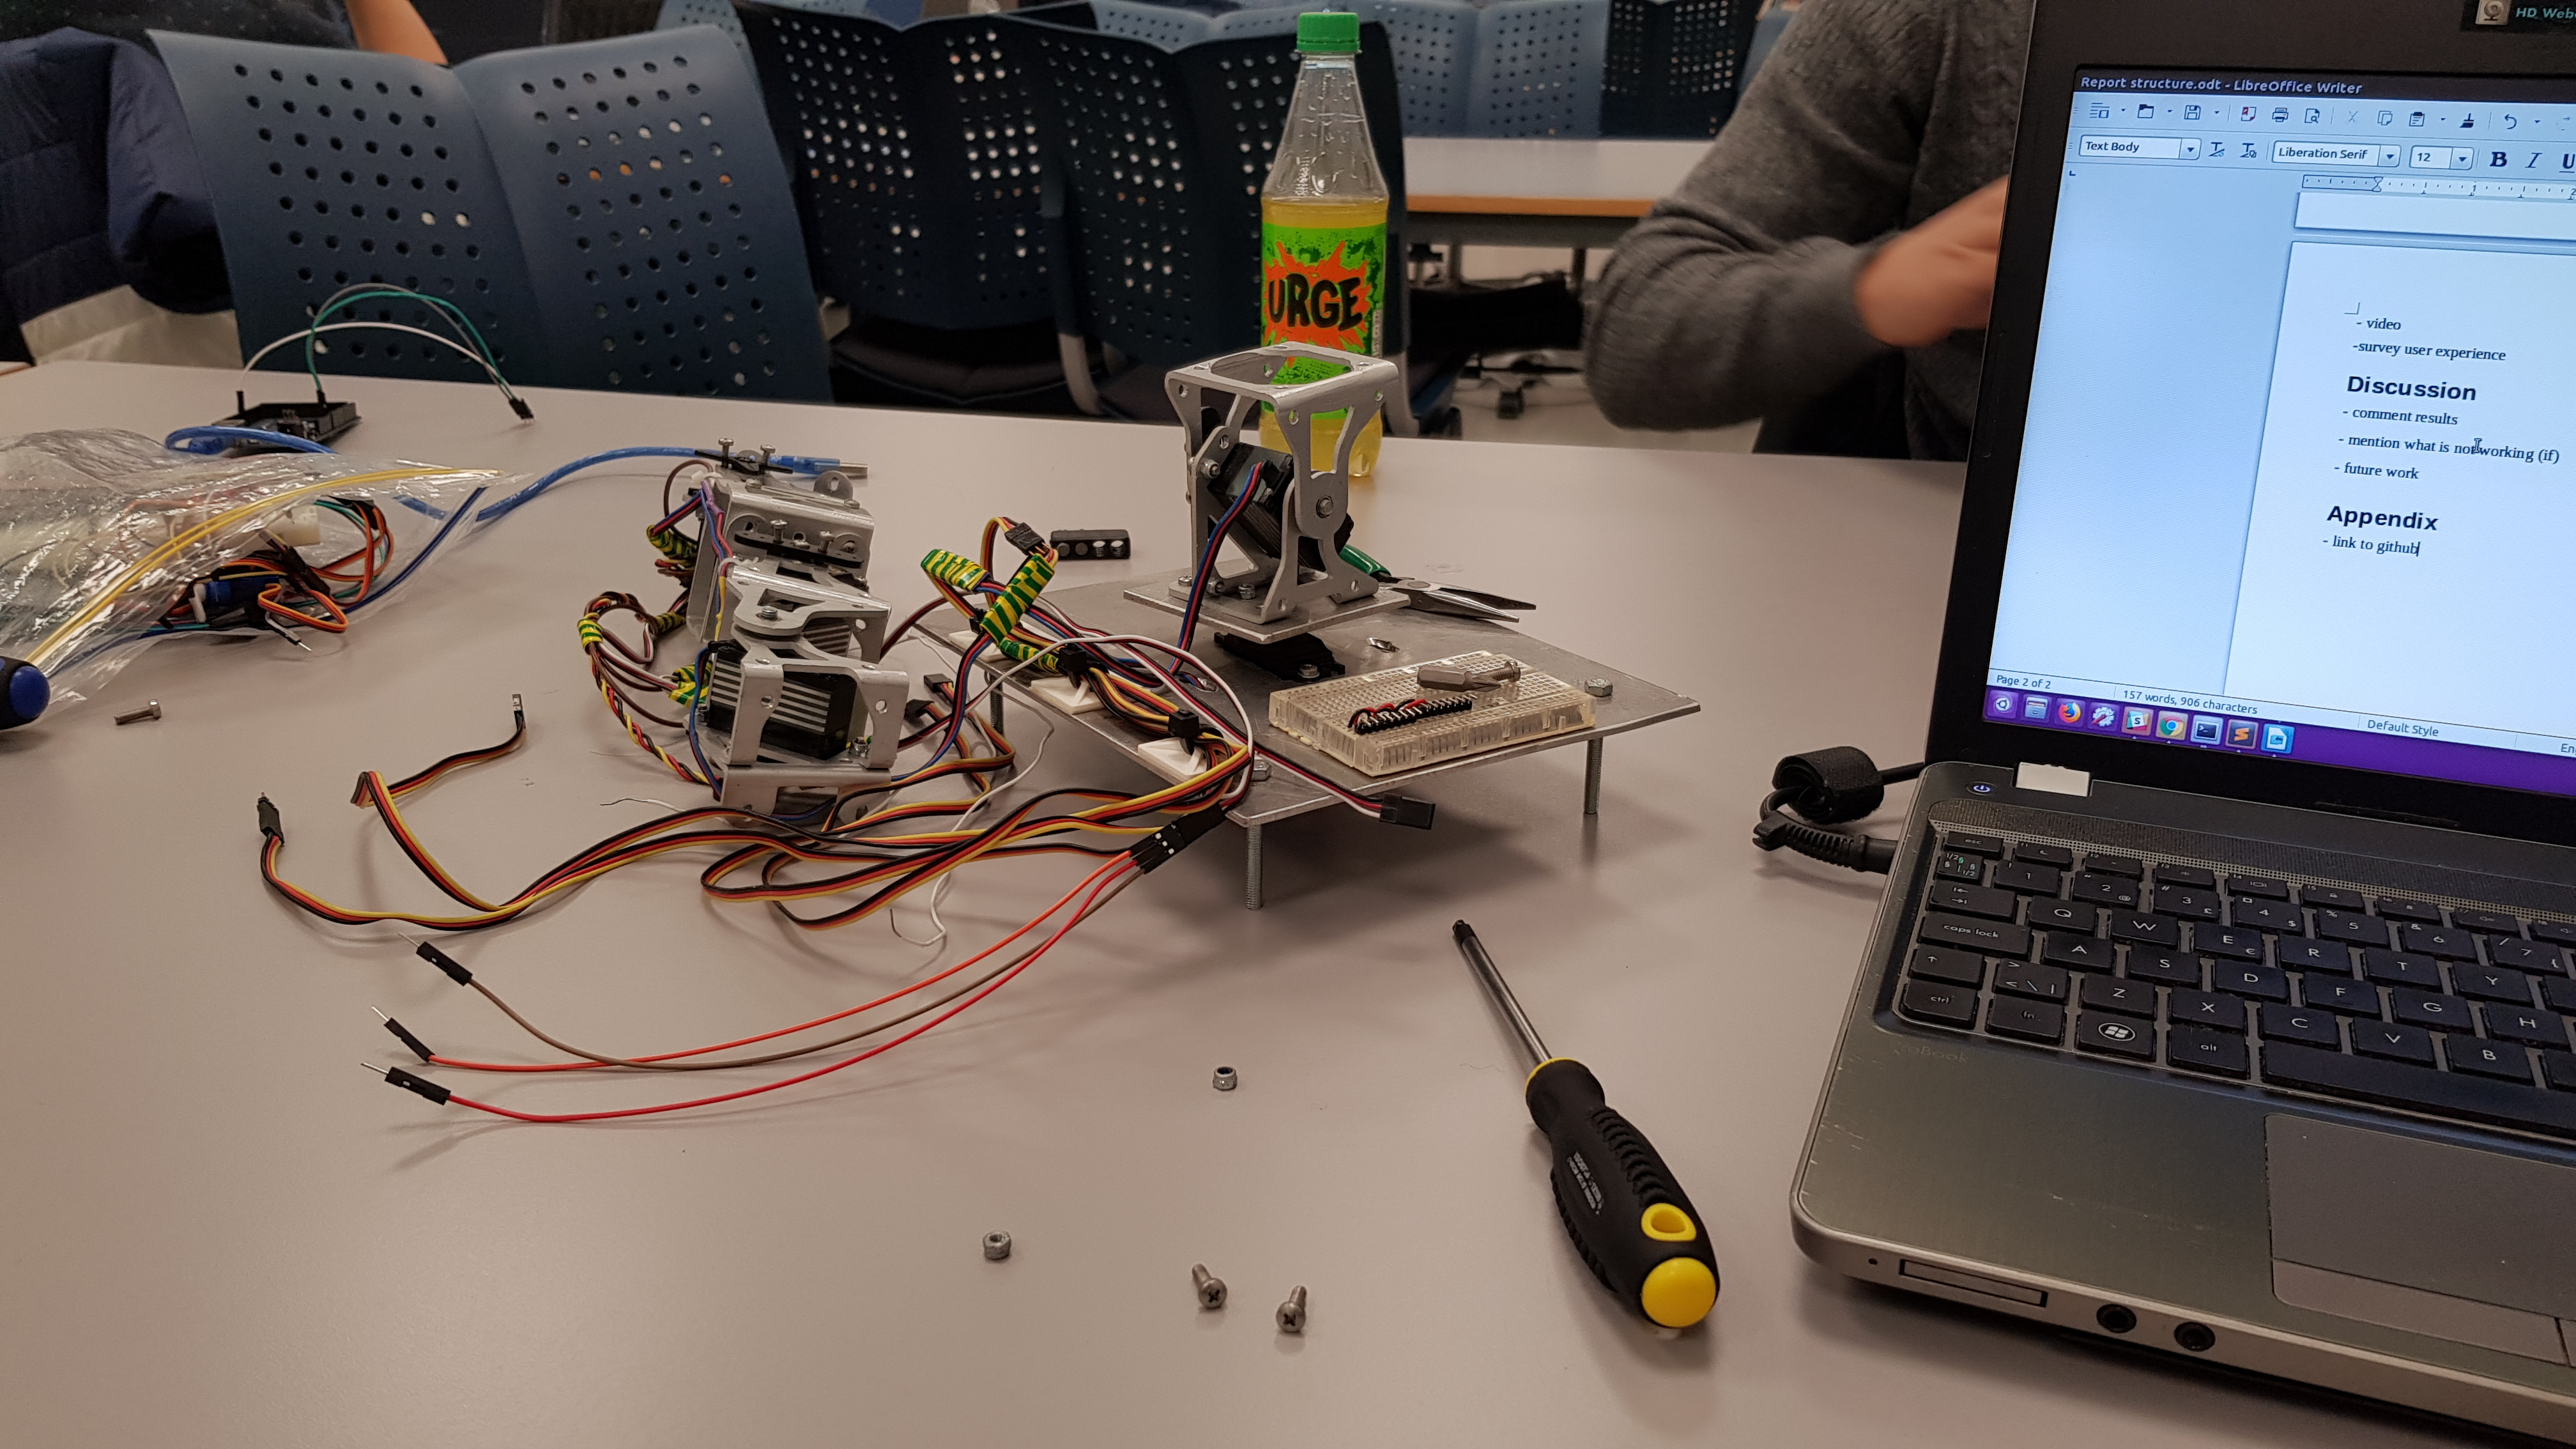
\includegraphics[width=0.8\linewidth]{../Diagrams/early-setup.jpg}
		\caption{Early stage of the hardware}
		\label{fig:early-rig}
	\end{figure}
	
	During the first tests of the robotic arm, we discovered that the torque would make the robot fall over. We decided to make a more stable mechanical rig, by attaching the robotic arm to a wooden platform. Figure \ref{fig:plank-rig} shows the process of making the wooden platform.

\begin{figure}[H]
\centering
\begin{subfigure}[b]{0.45\linewidth}
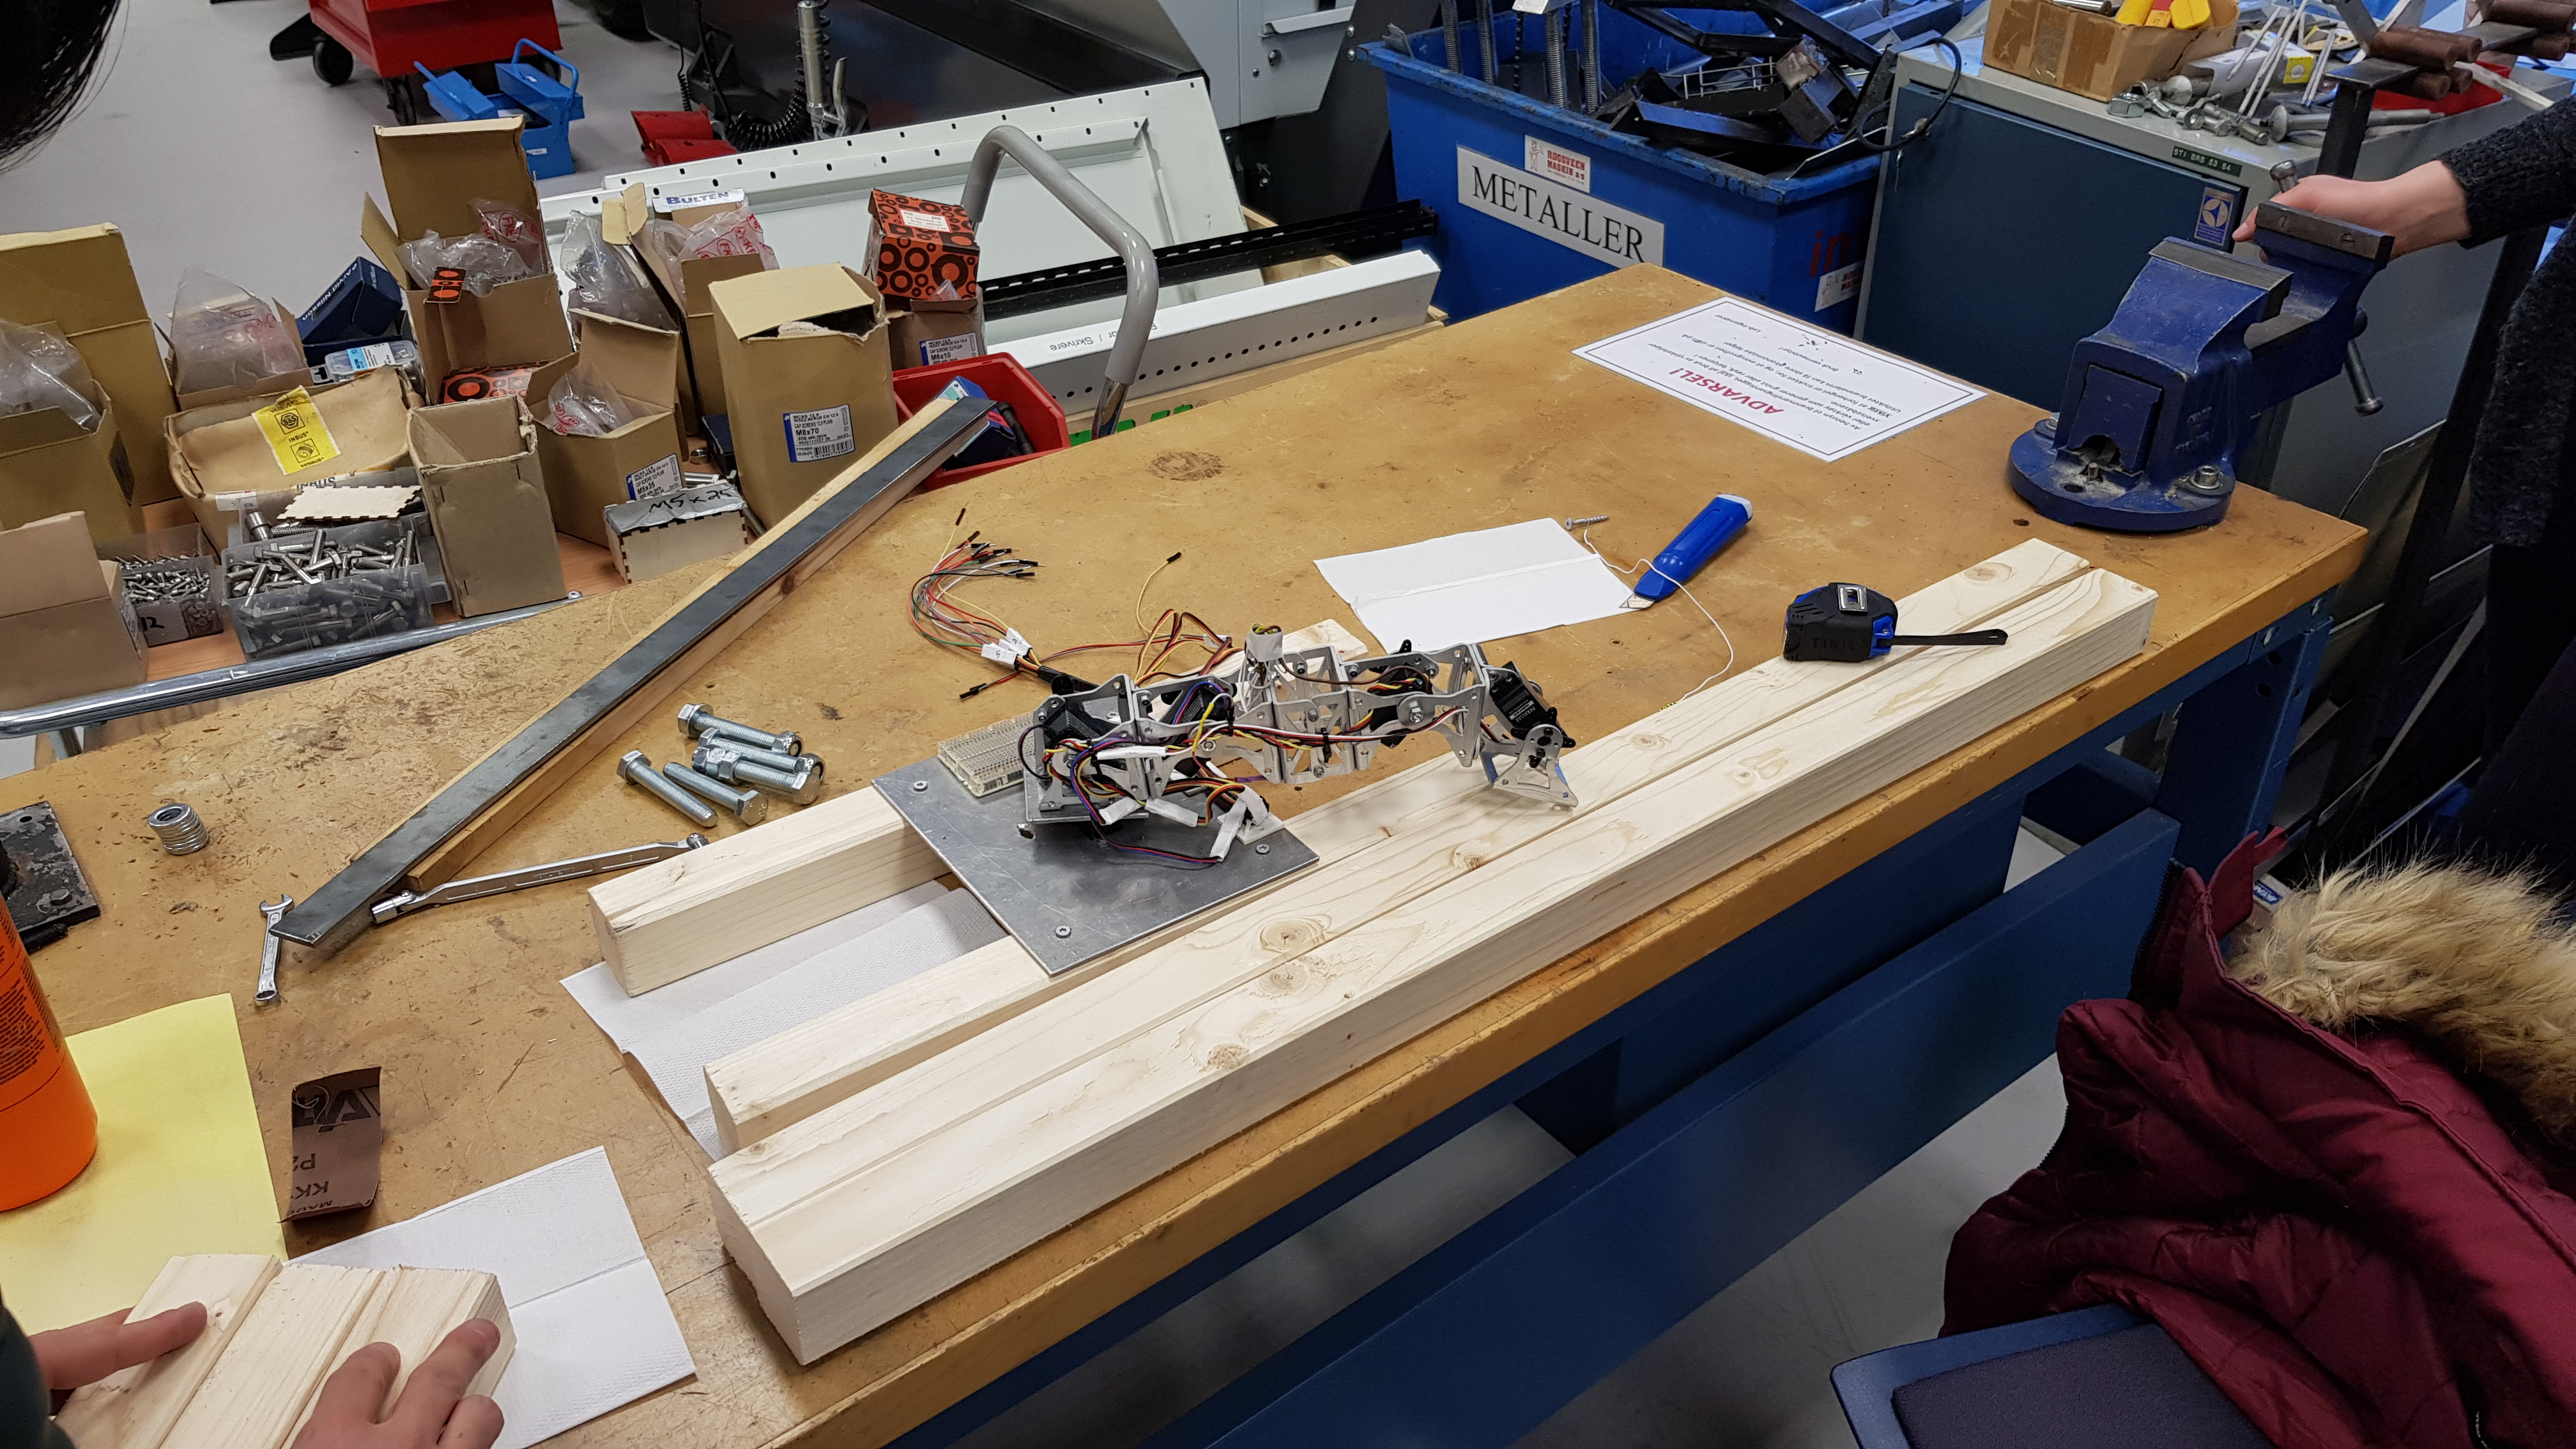
\includegraphics[width=\textwidth]{../Diagrams/plank1.jpg}
\caption{Planning}                		
\end{subfigure}
\begin{subfigure}[b]{0.45\linewidth}
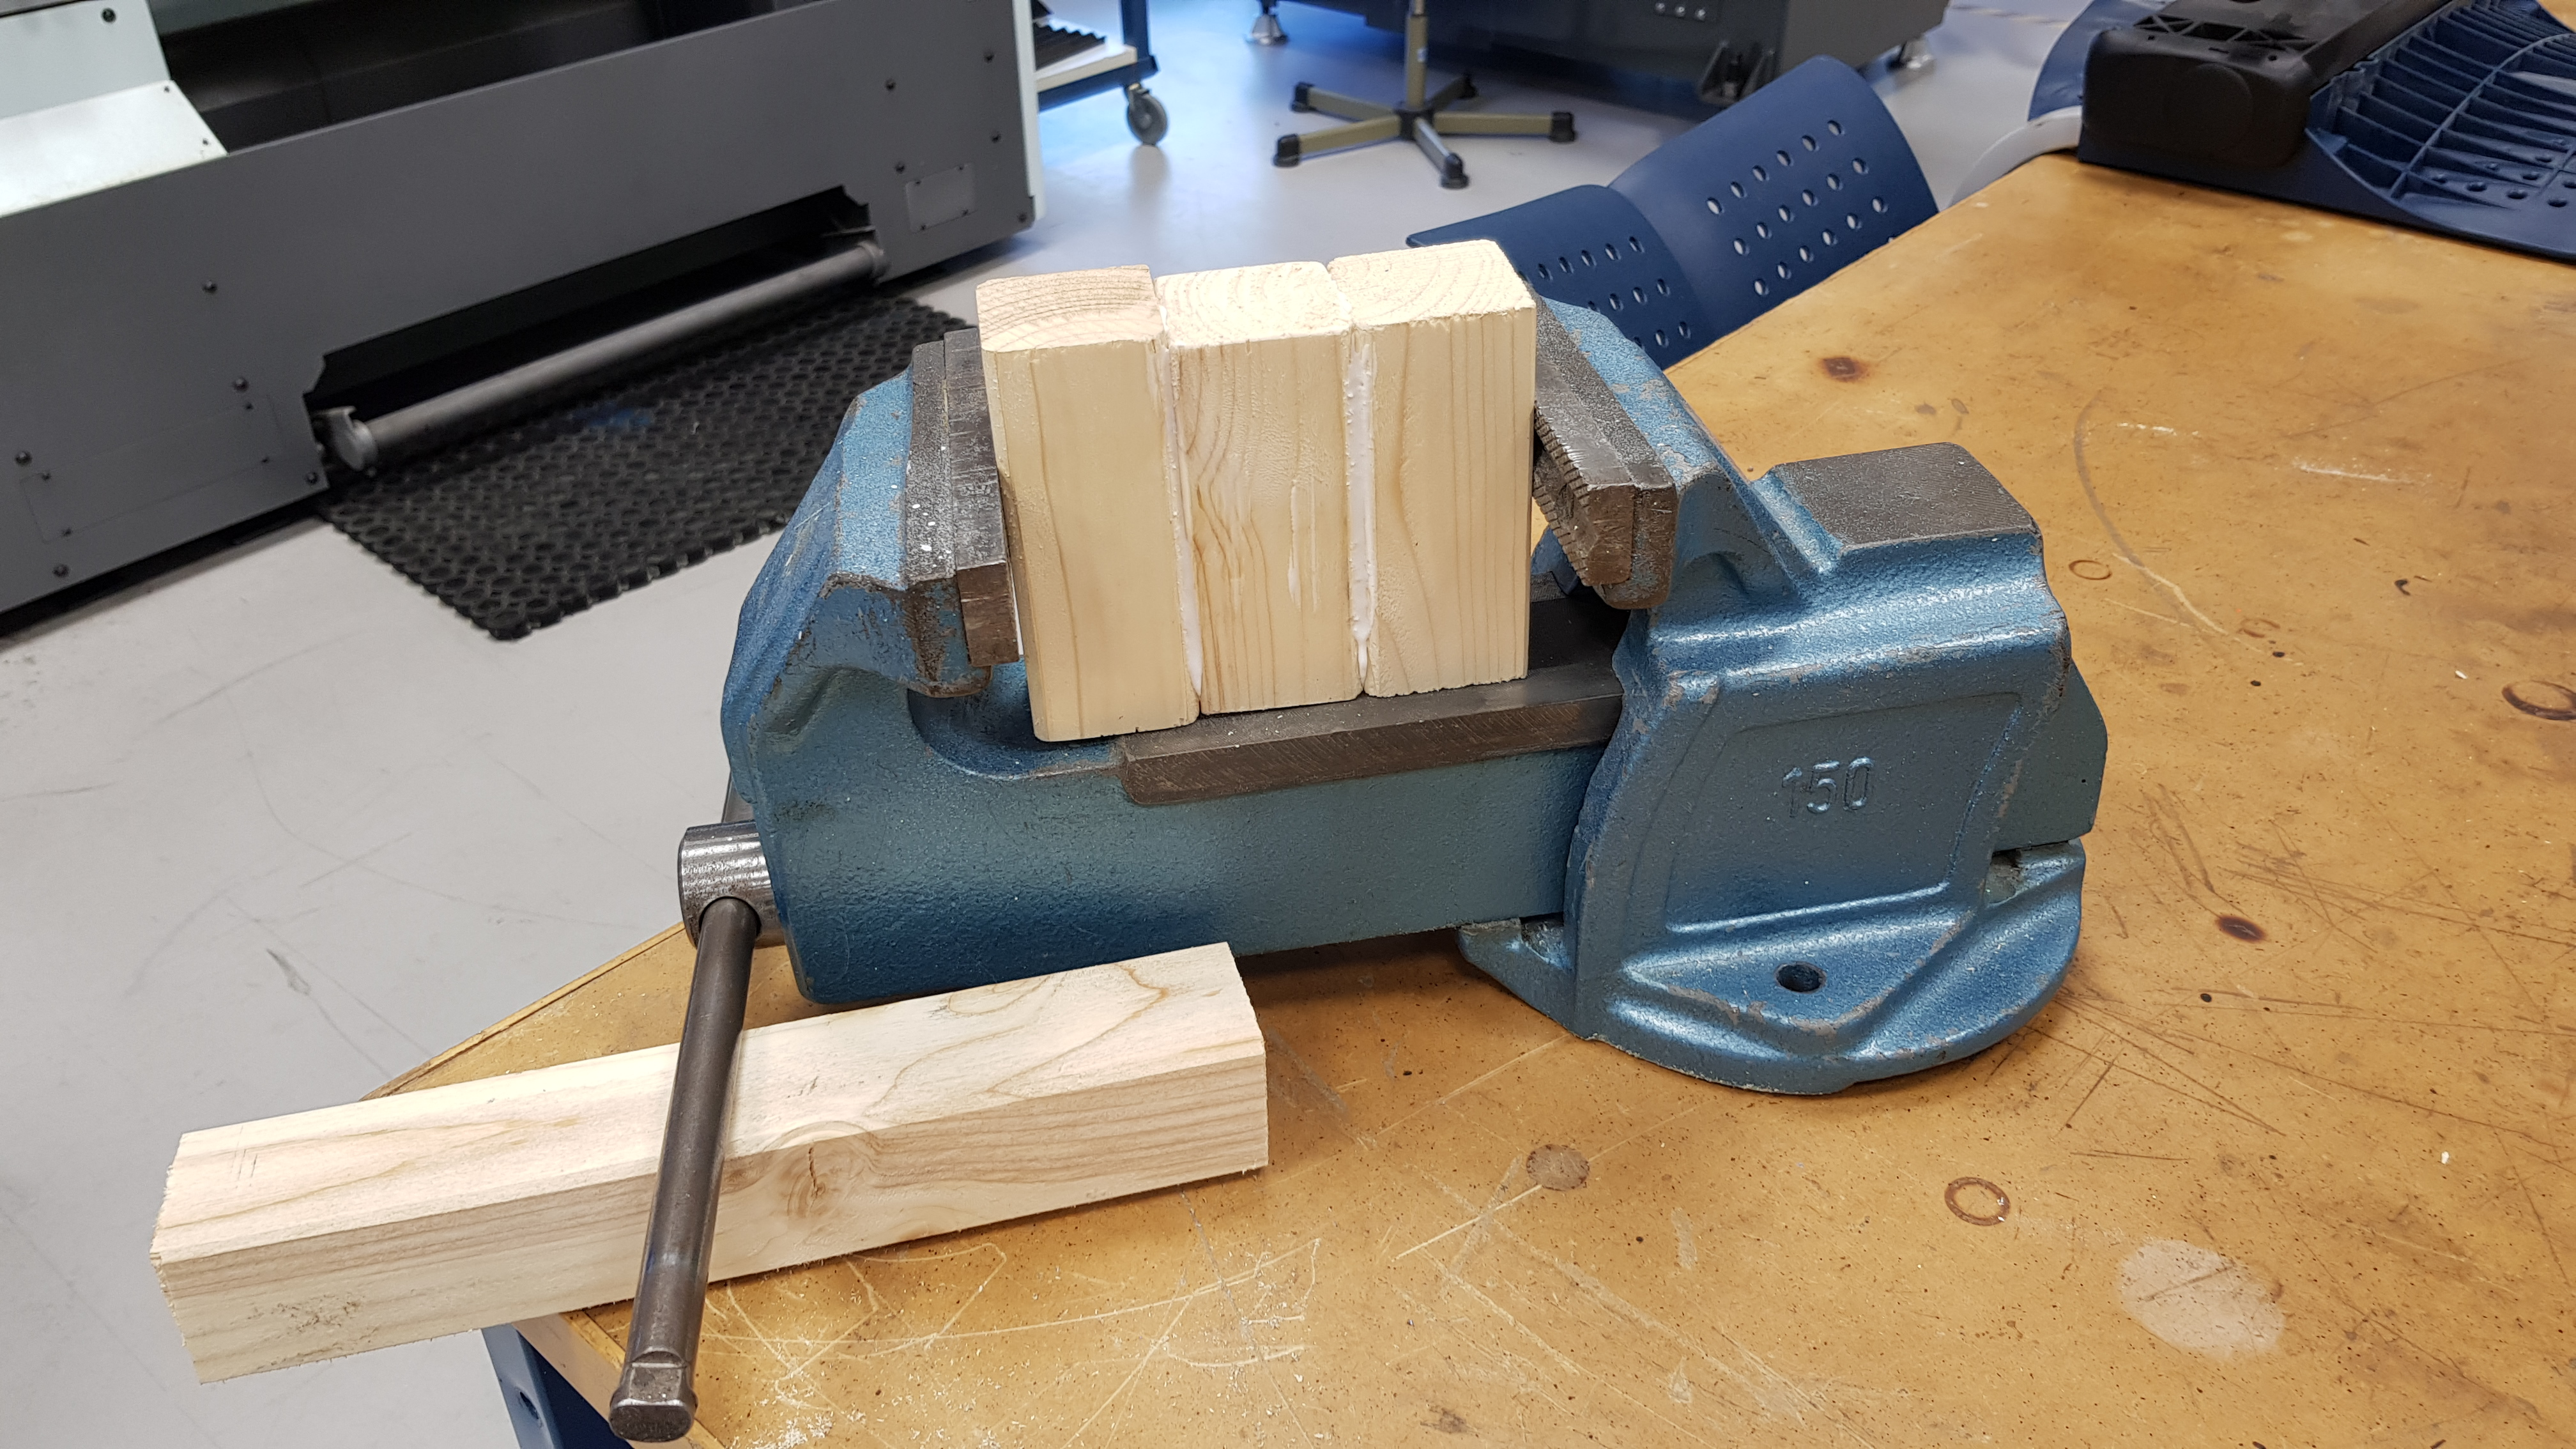
\includegraphics[width=\textwidth]{../Diagrams/plank2.jpg}  
\caption{Adjusting}              		
\end{subfigure}
\begin{subfigure}[b]{0.45\linewidth}
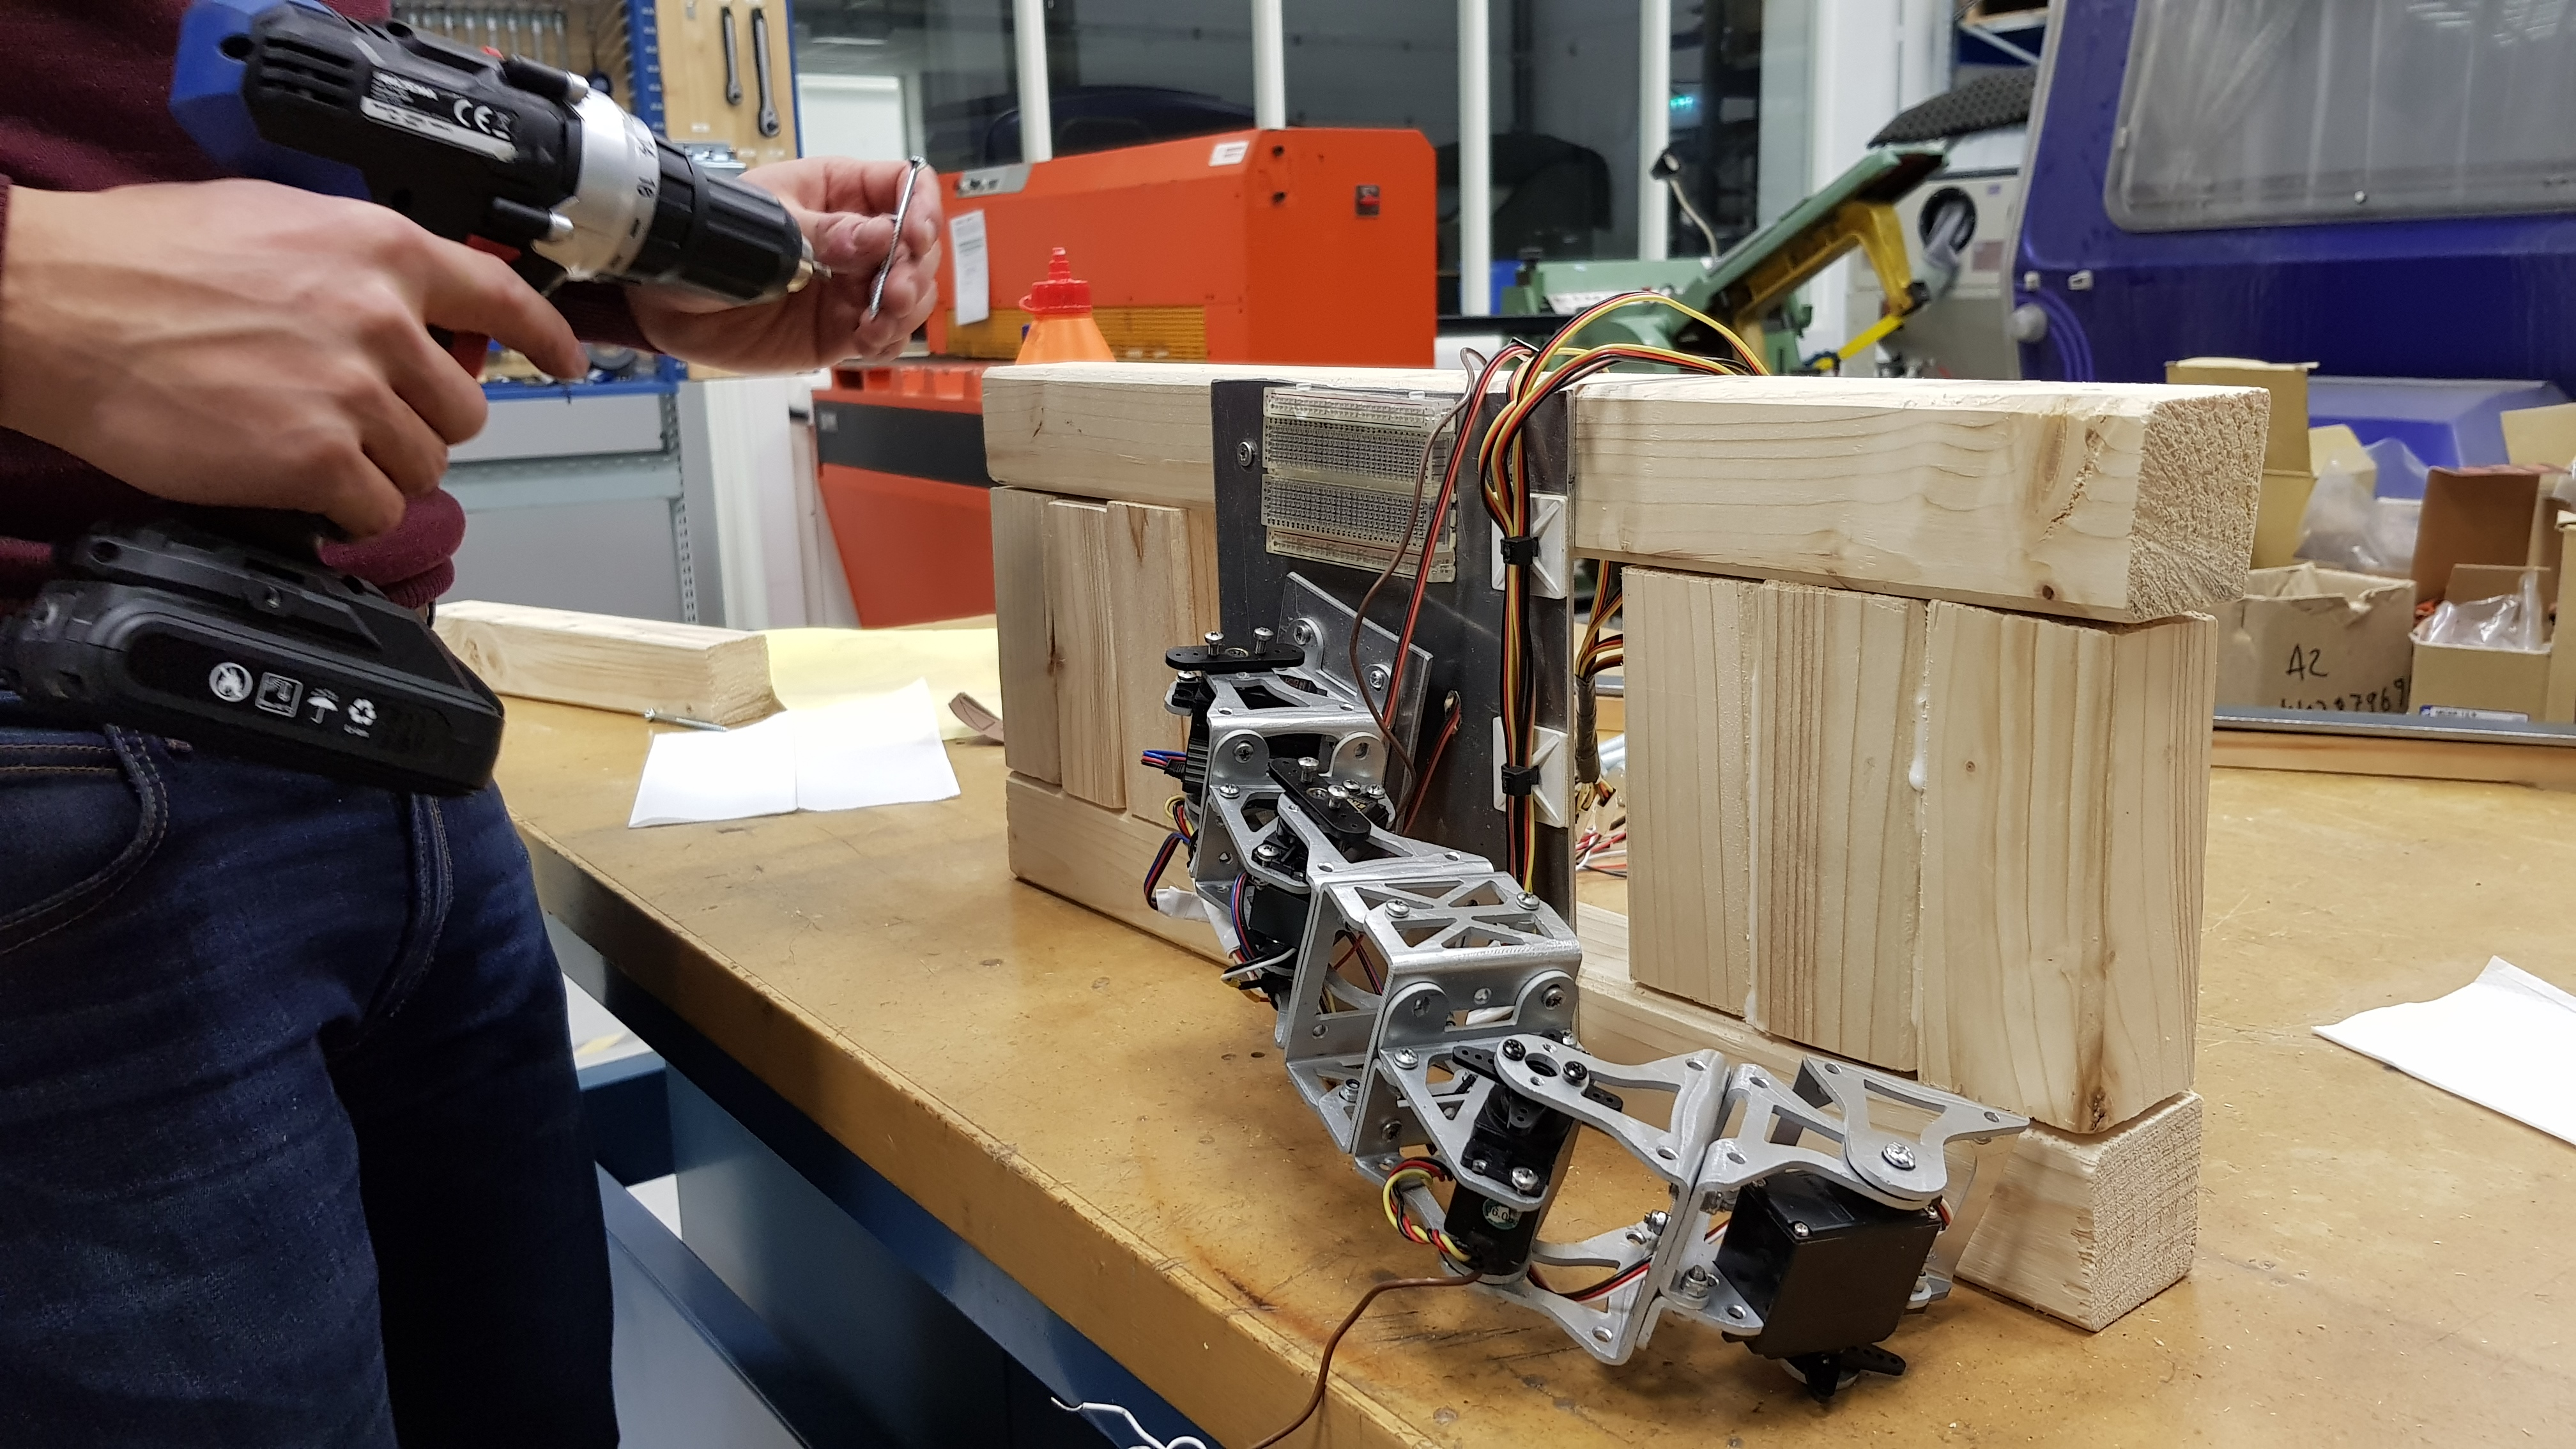
\includegraphics[width=\textwidth]{../Diagrams/plank3.jpg}  
\caption{Assembly}              		
\end{subfigure}
\begin{subfigure}[b]{0.45\linewidth}
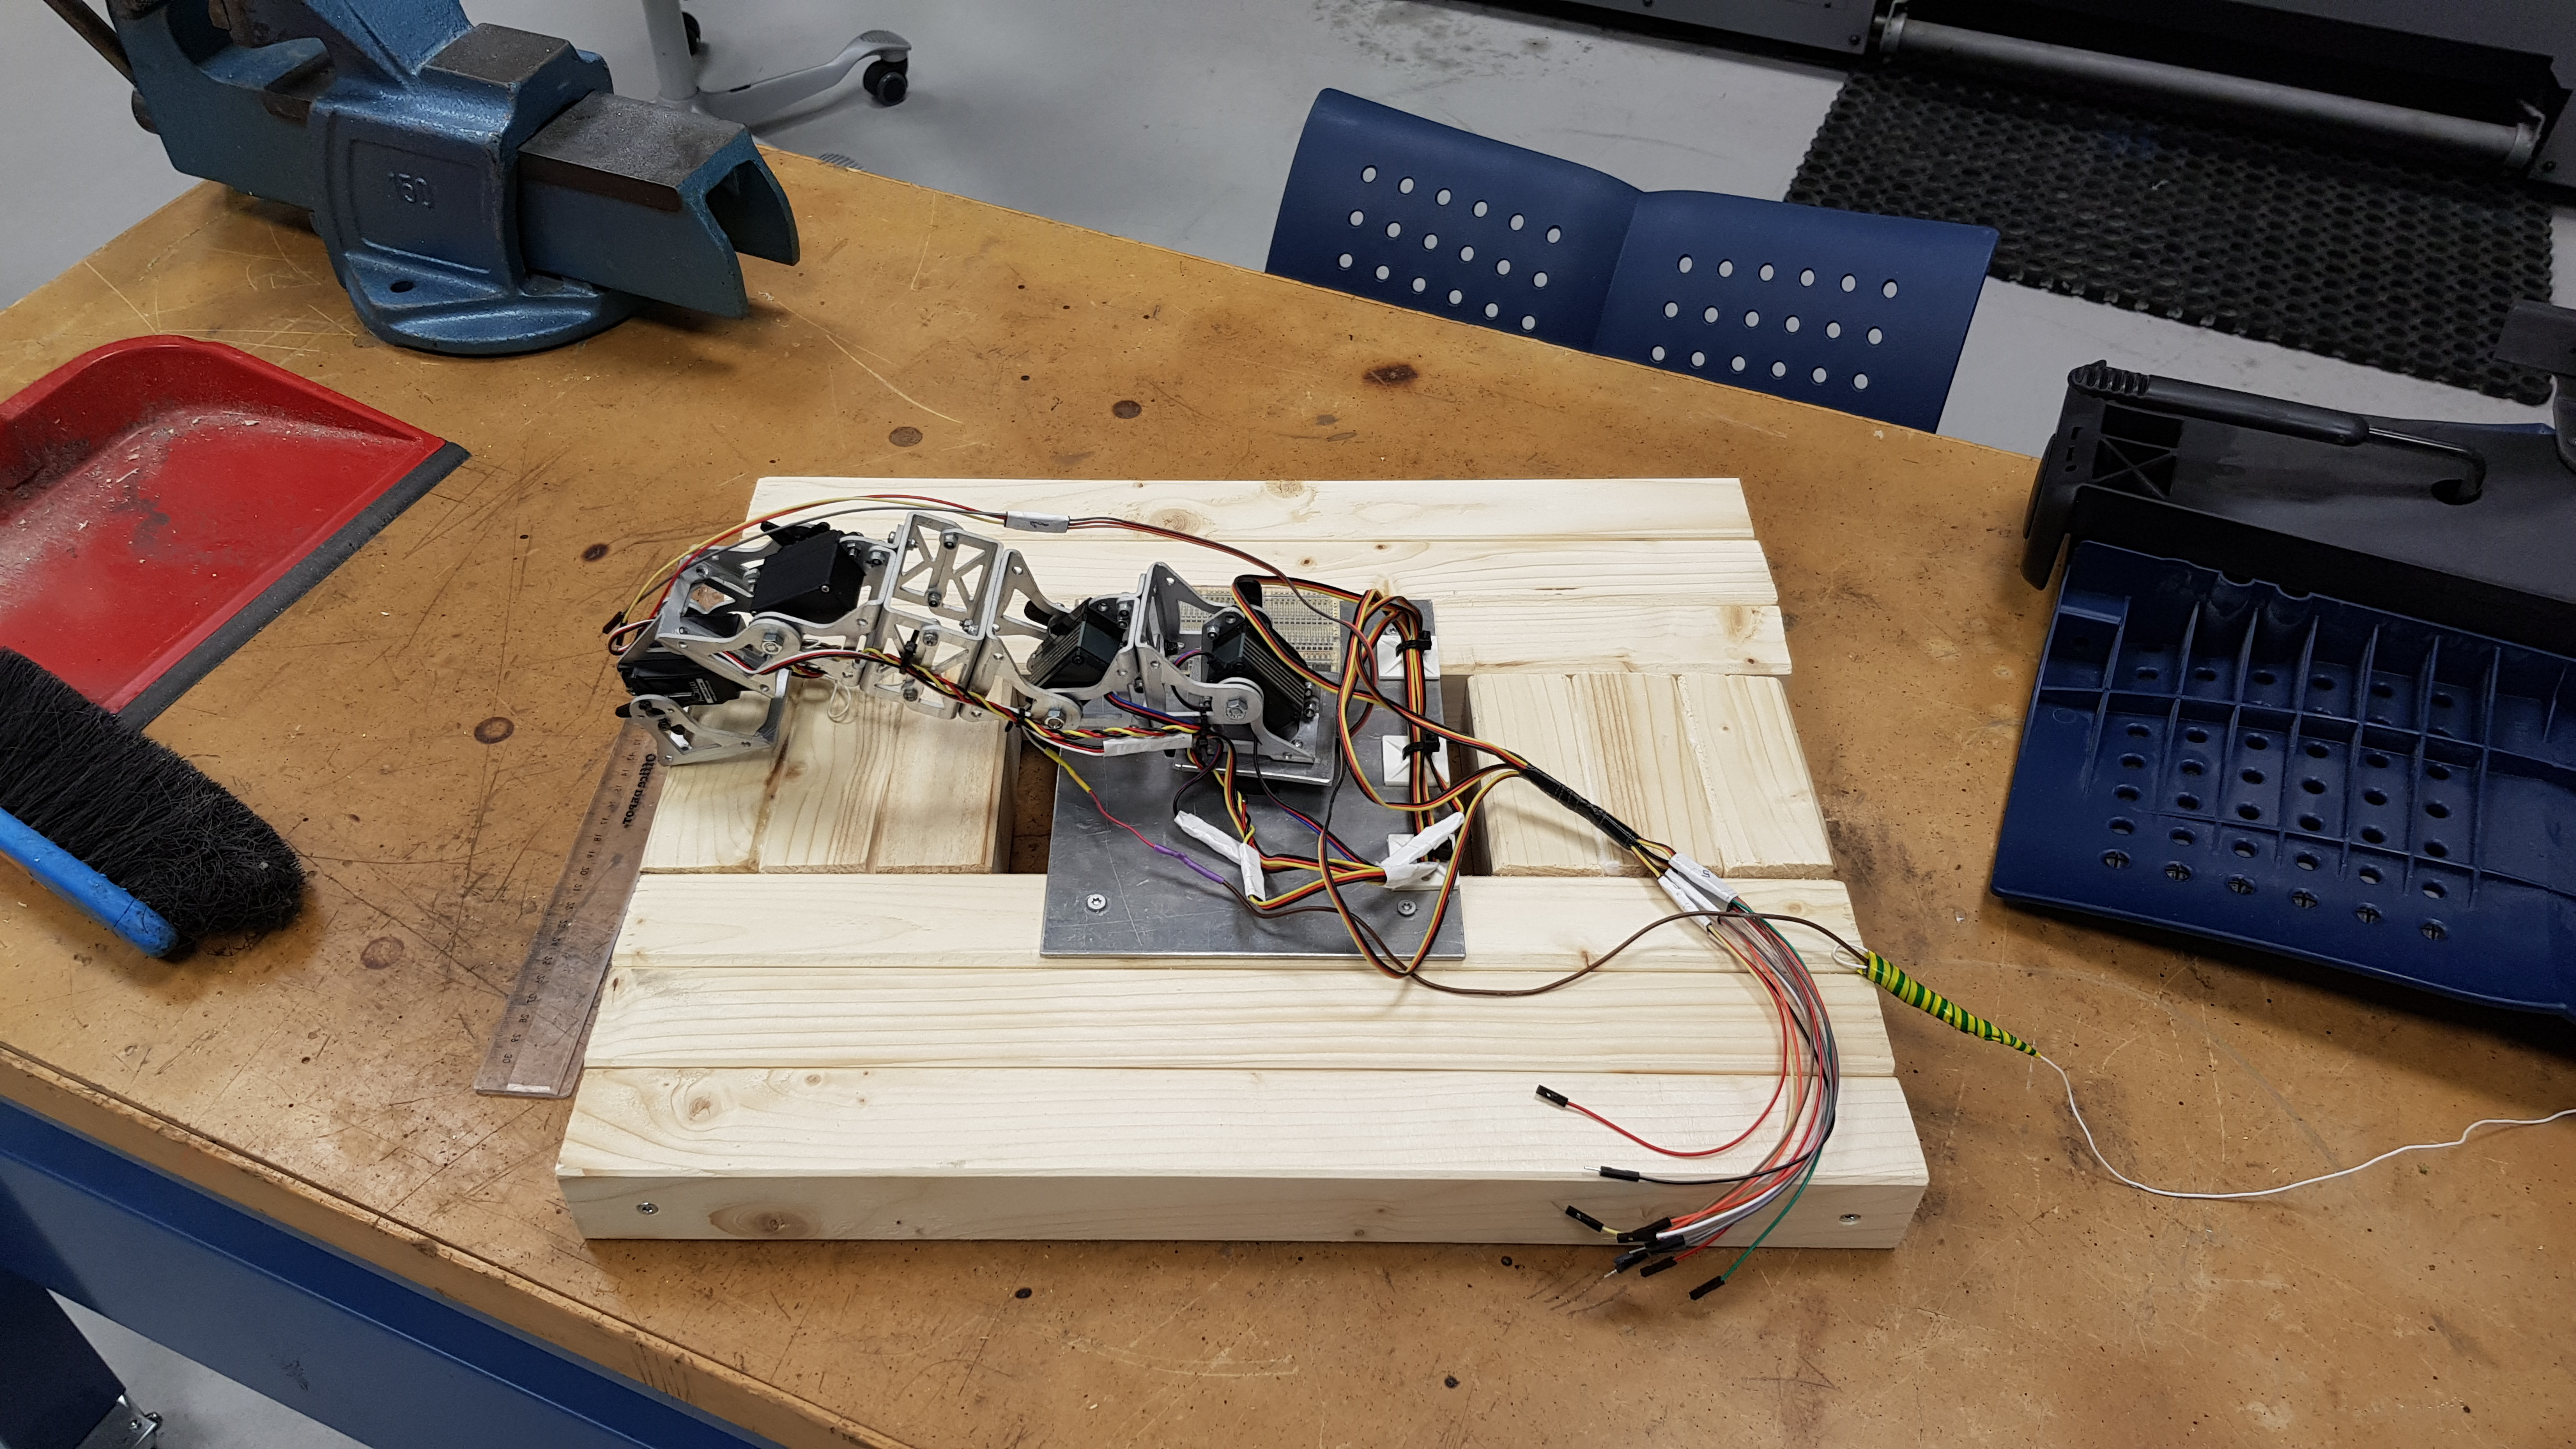
\includegraphics[width=\textwidth]{../Diagrams/plank4.jpg}  
\caption{Finished}              		
\end{subfigure}
\caption{Process of making the wooden rig}
\label{fig:plank-rig}
\end{figure}

	\subsubsection{Power supply}
	\label{power}
	The servo motors are running nominally at 6V. As the arm consists of five motors, we could not power them all from the Arduino. We decided to buy battery holders to run 4 AA batteries in series. Since an AA battery is 1.5V, running four of them in series adds up to 6V.
	
	Due to the bigger torque applied to the bottom motors, we decided to supply the bottom three motors with 6V each,  having them operate at nominal voltage level. The upper two motors of the arm are powered by one Arduino each, meaning they get 5V. Figure \ref{fig:power} shows the power supply used in ARPA. Note that the battery on the right holds six more batteries under the ones showed.
	
	\begin{figure}[H]
		\centering
		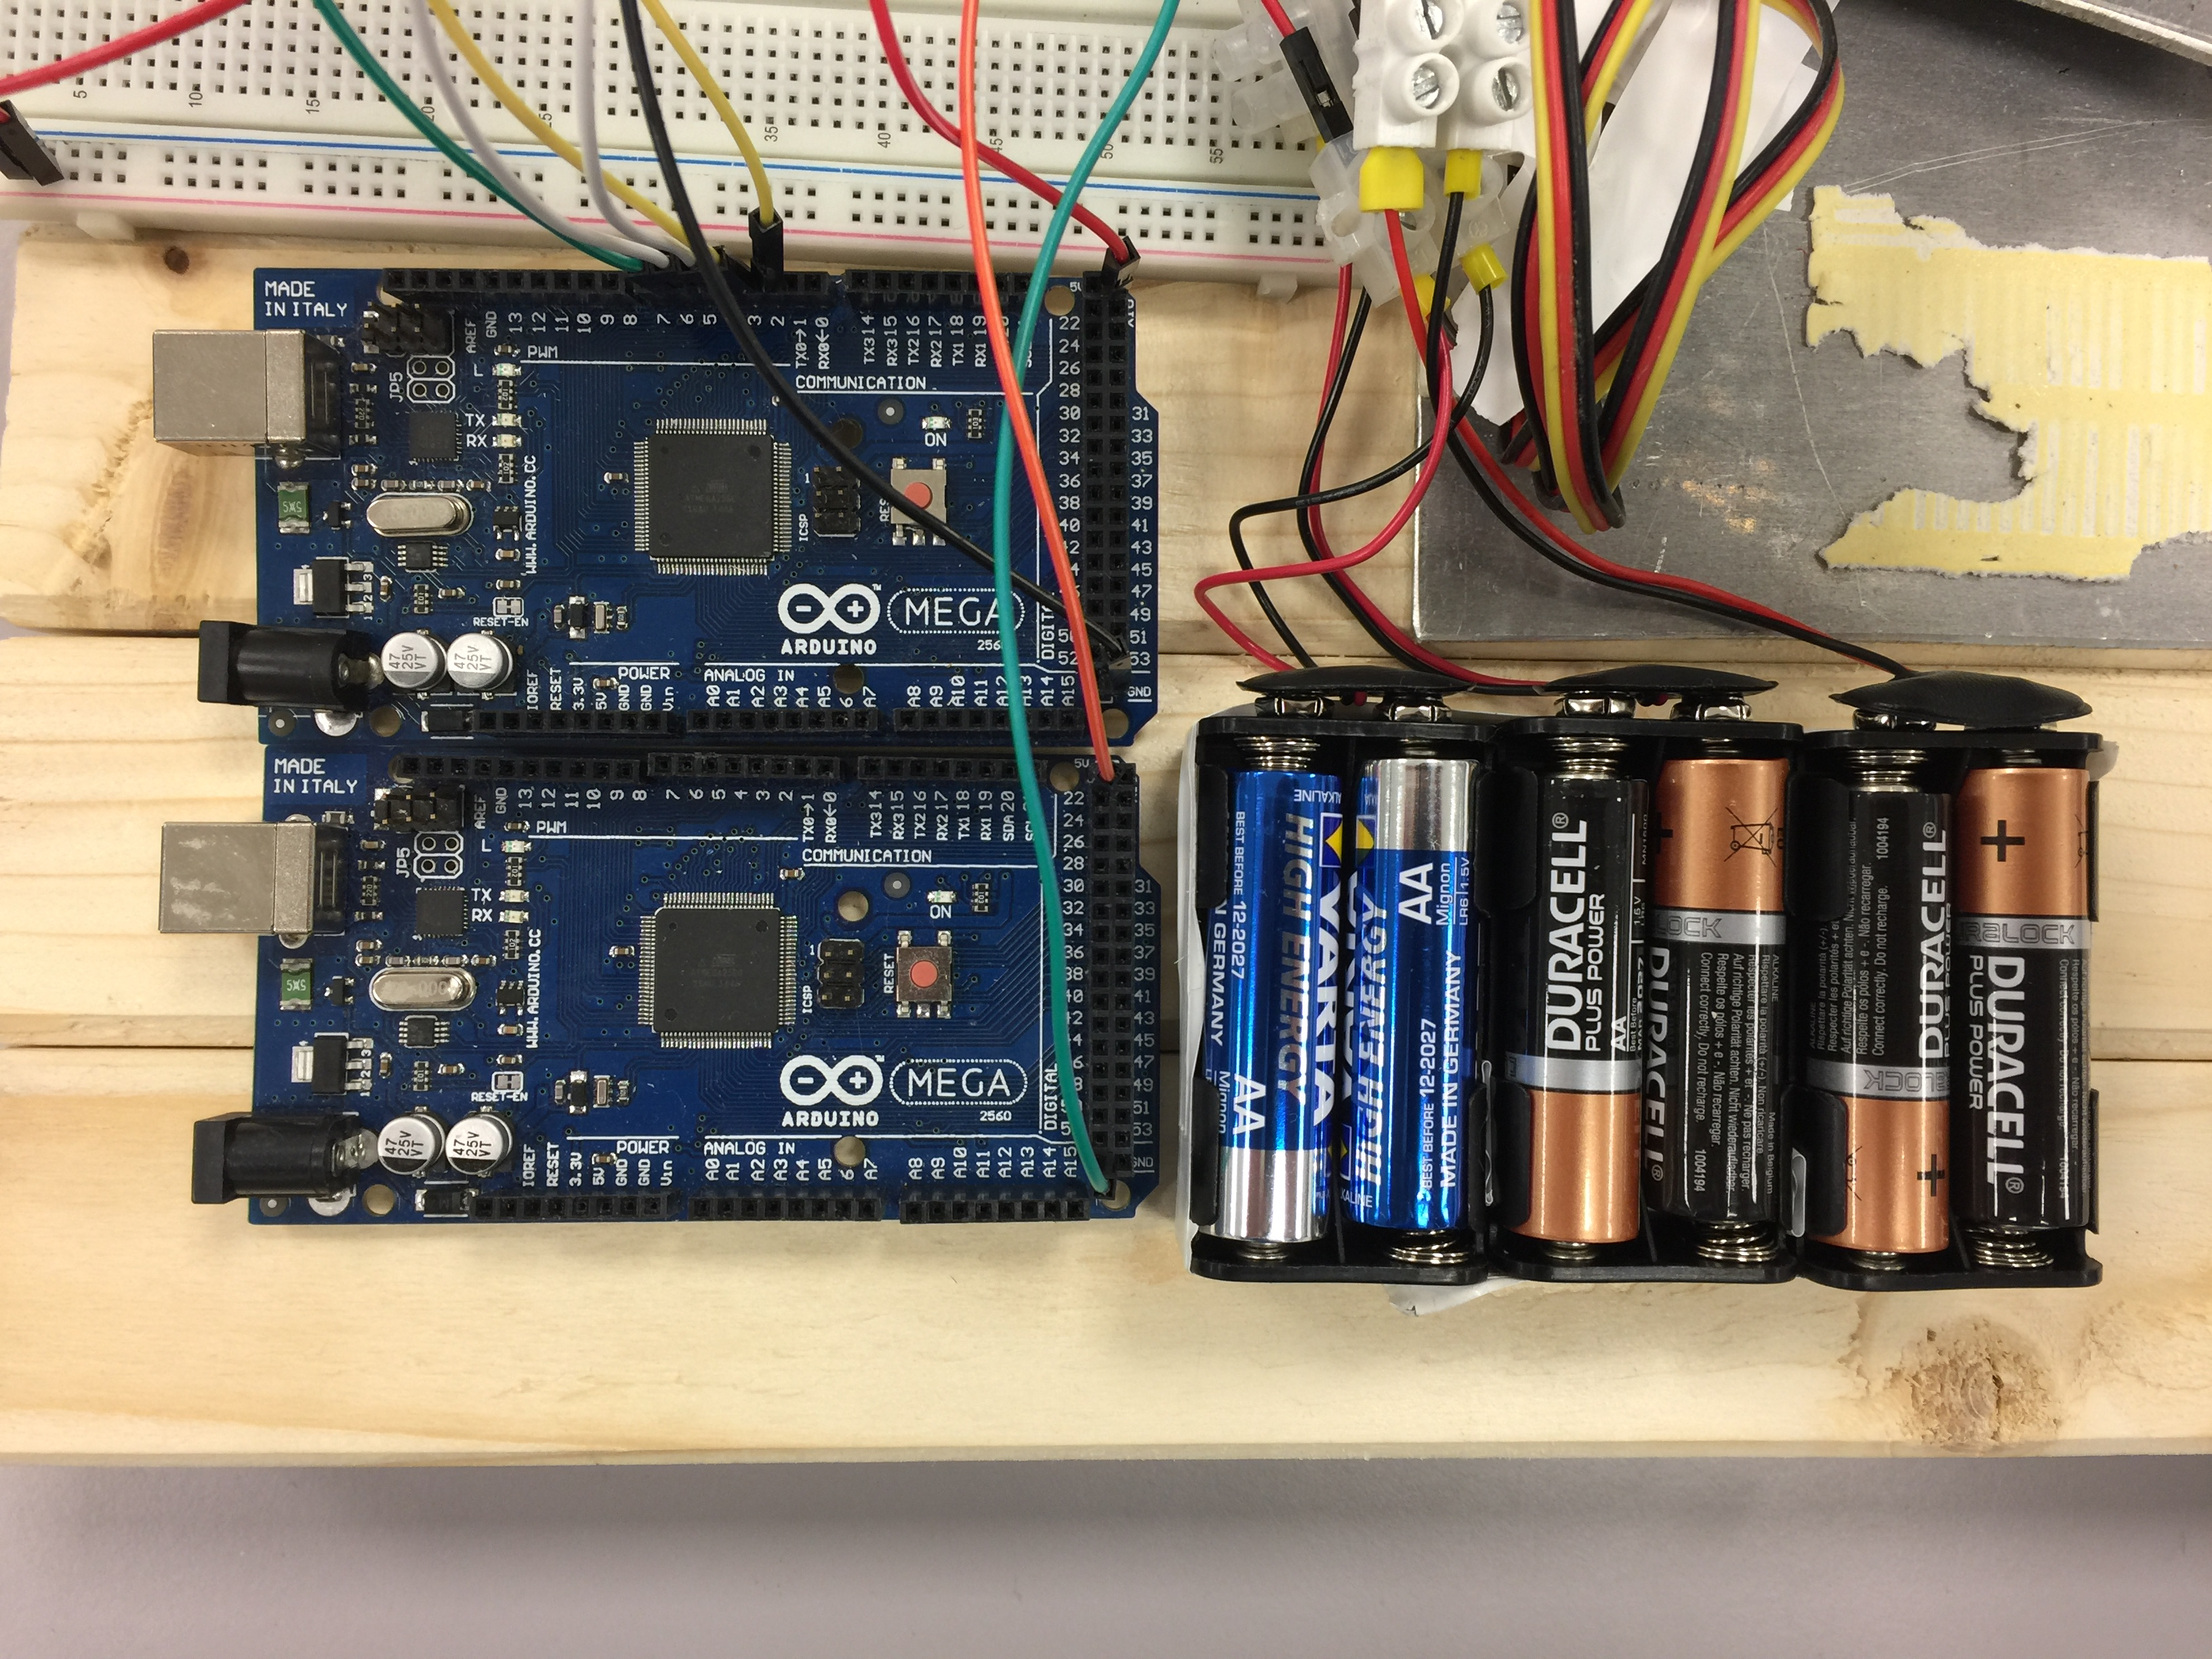
\includegraphics[width=0.8\linewidth]{../Diagrams/PowerSupply.jpg}
		\caption{Power supply setup}
		\label{fig:power}
	\end{figure}
	
	\subsubsection{Arduino wiring}
	Figure \ref{fig:wiring} shows the wiring of Arduino to supply power to the motors, as well as controlling them with PWM signals.
	
	\begin{figure}[H]
		\centering
		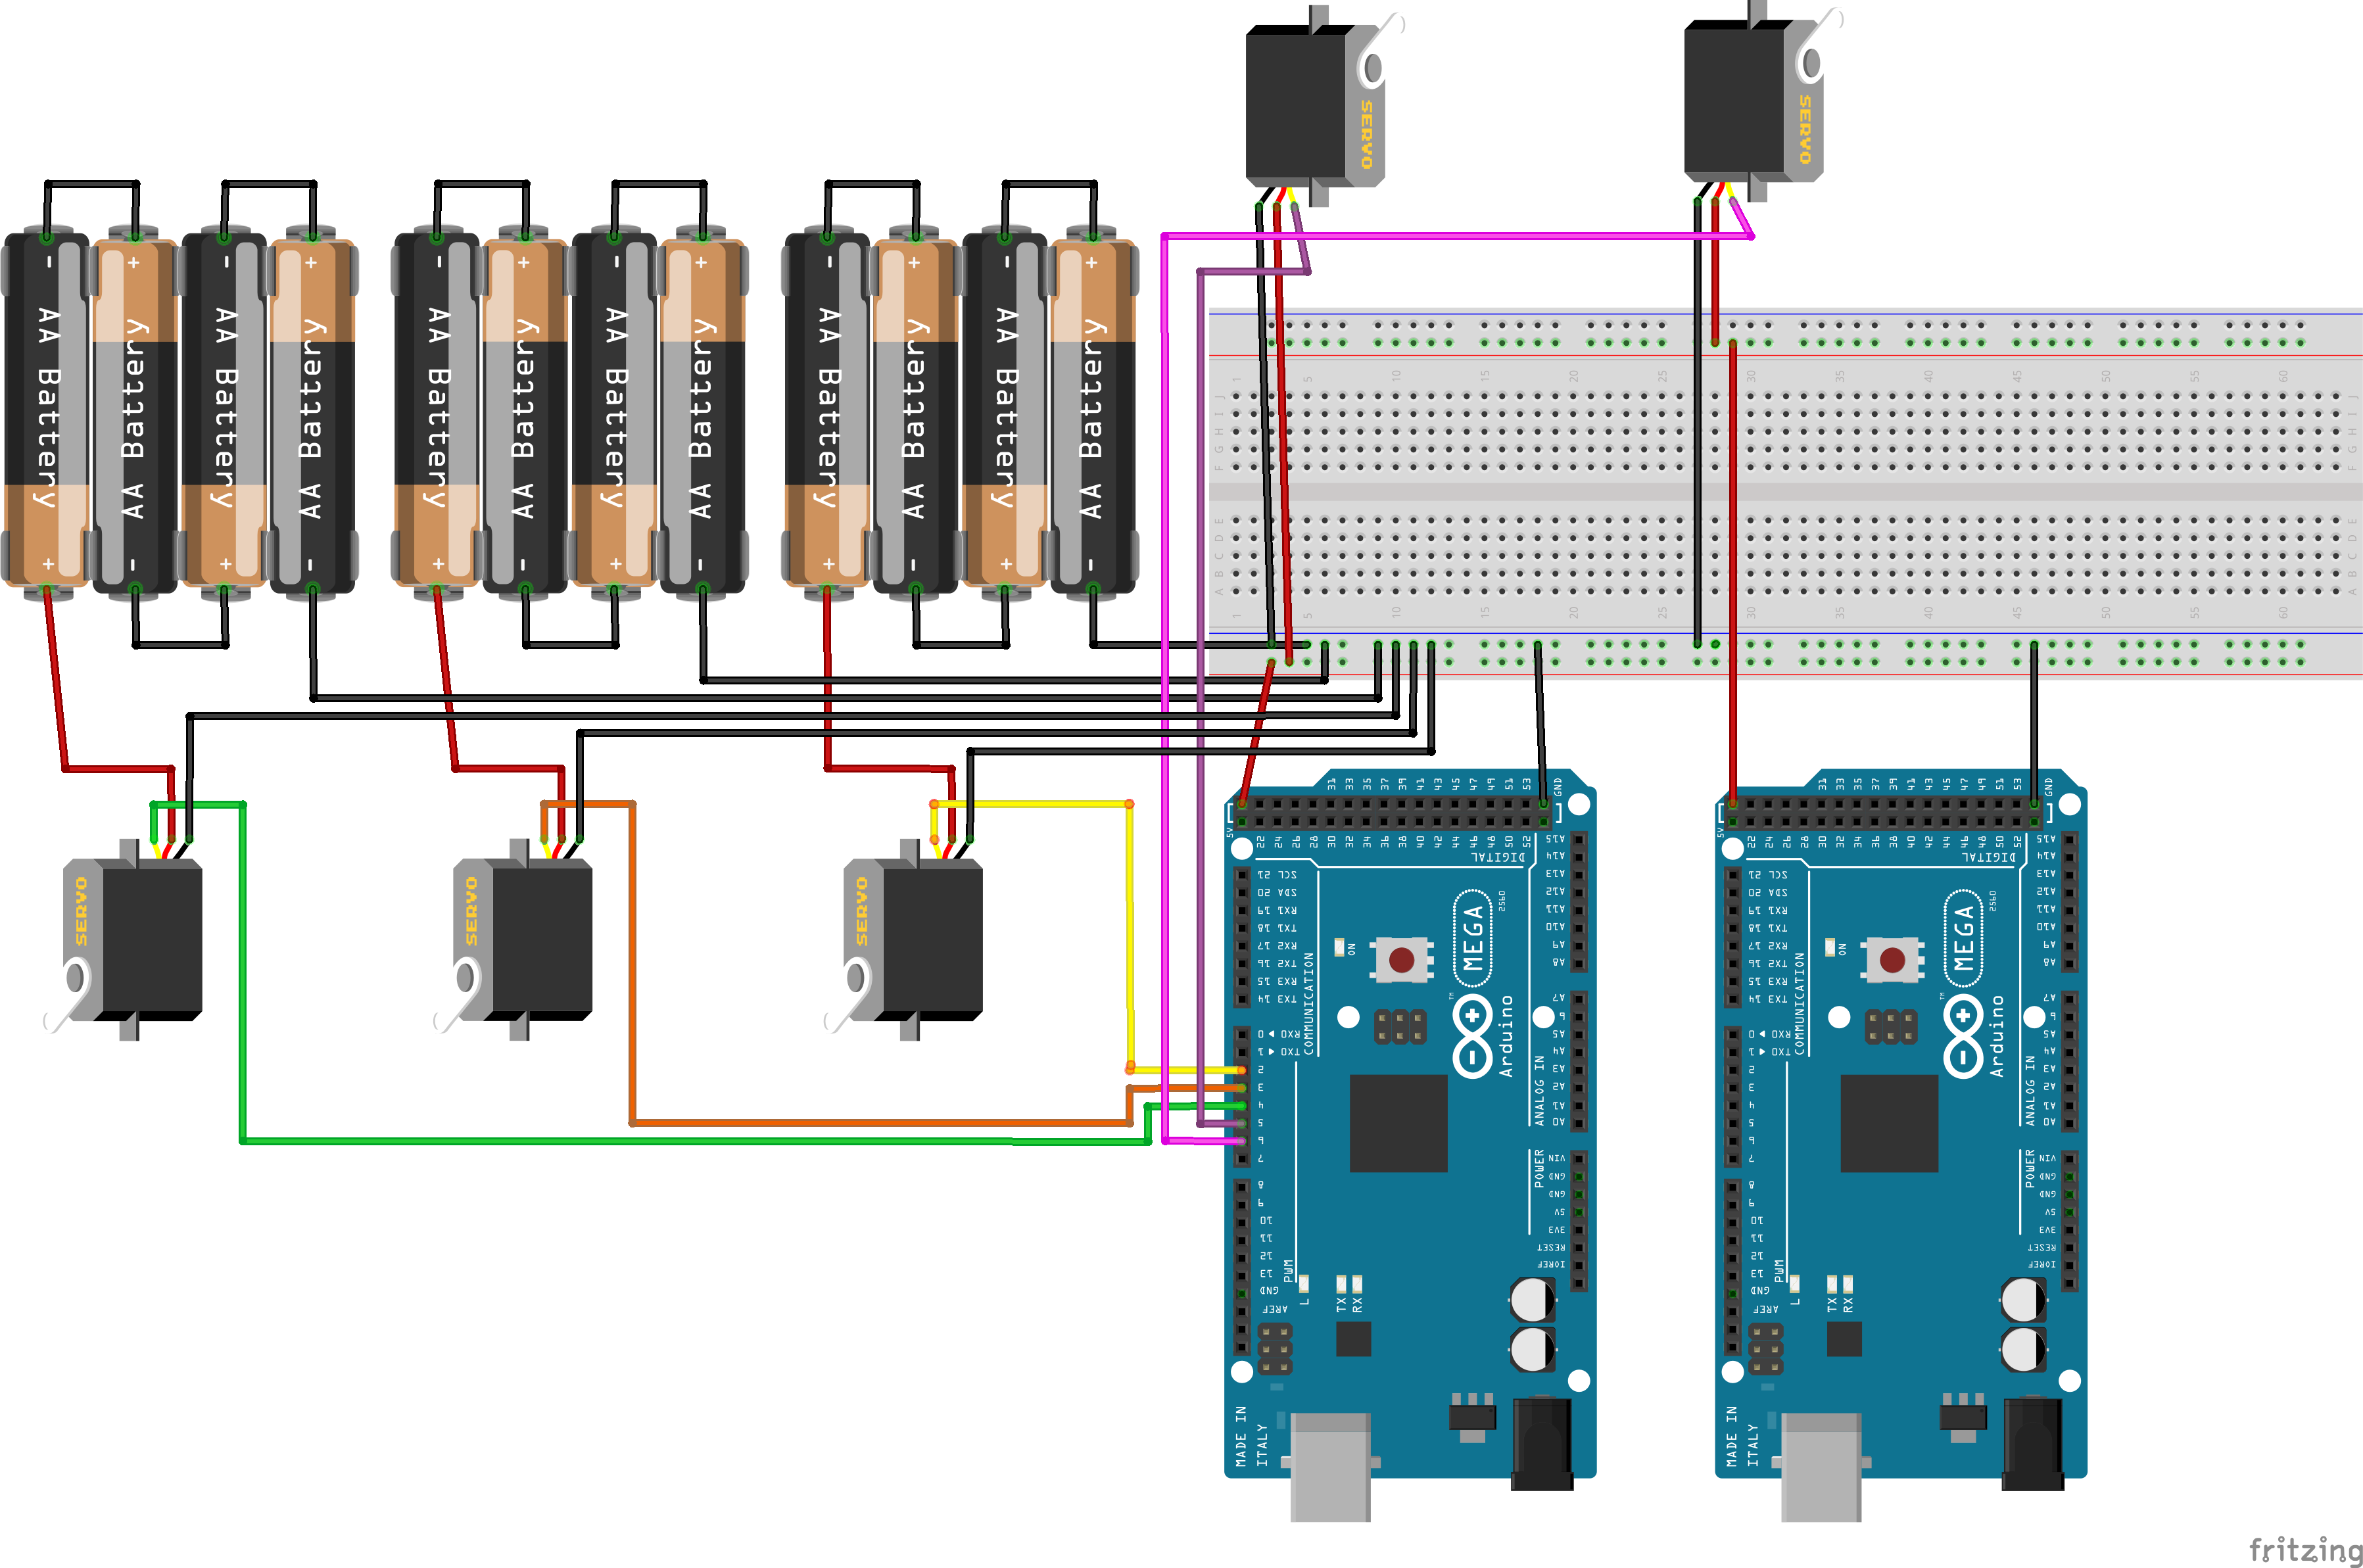
\includegraphics[width=0.8\linewidth]{../Diagrams/Wiring.png}
		\caption{Arduino wiring}
		\label{fig:wiring}
	\end{figure}
	
		
	\section{Simulation and experiments}
	\label{simex}
	Since the project has served as a introduction to many new tools, we have had several experiment along the way to learn how to use these tools. This section will go through the simulations and experiments we have conducted during the course of the project.
	
	\subsection{Arduino knob}
	The first experiment was to learn how to control the servo motors. We used a couple of approaches, one being to control the servo motors by the output of a potentiometer. It was a quick process, which allowed us to move onto bigger challenges.
	
	\subsection{ROS Turtlesim}
	The next stage in the project was to learn the ROS ecosystem. ROS has quite a steep learning curve, and much time was spent just getting a basic understanding of all the fundamentals. One specific experiment was the turtlesim tutorial found in \cite{turtle2017}. This tutorial gave a good insight into the ROS graph concept, i.e. the separation of functionality into nodes.
	
	\subsection{Arduino subscriber}
	After getting a grip of the basics in ROS, we went on to integrating the Arduino into the ROS node network. The goal of this experiment was to setup a subscriber on the Arduino which receives a joint angle that it writes to a servo motor. This experiment was successful as we managed to rotate the servo by publishing a message from the terminal on the computer.
	
	\subsection{Initial modeling}
	The next experiment in the project was to get a simple robotic model visualized in Gazebo. Through guidance in \cite{joseph2015}, we were able to get a simple representation of the robotic arm with the correct amount of joints and links, but without precise D-H parameters. We managed to make this model subscribe to the same topics subscribed to by the Arduino so the joints in the simulated world received the same messages as the servo motors on the physical robot. Figure \ref{fig:init-model} shows the initial model of the robotic arm.
	
	\begin{figure}[H]
		\centering
		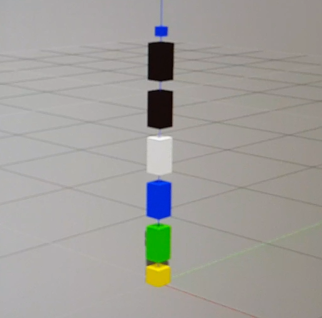
\includegraphics[width=0.5\linewidth]{../Diagrams/URDF-first.png}
		\caption{Initial model}
		\label{fig:init-model}
	\end{figure}
	
	\subsection{Inverse kinematics}
	\label{invkin}
	To convert Cartesian coordinates to joint space, we needed to find the inverse kinematics of the robotic arm. We used a symbolic approach to first derive the forward equation of the geometric representation shown in figure \ref{fig:geometric} follow by the solving of the inverse kinematics. The resulting equations for $\theta_1,\,\theta_2,\,\theta_3,\,\theta_4,\,\theta_5$ are shown below. The mathematics in its entirety is appended as appendix \textit{\ref{appendix:ik} Complete kinematic solution}.
	
	\begin{figure}[H]
		\centering
		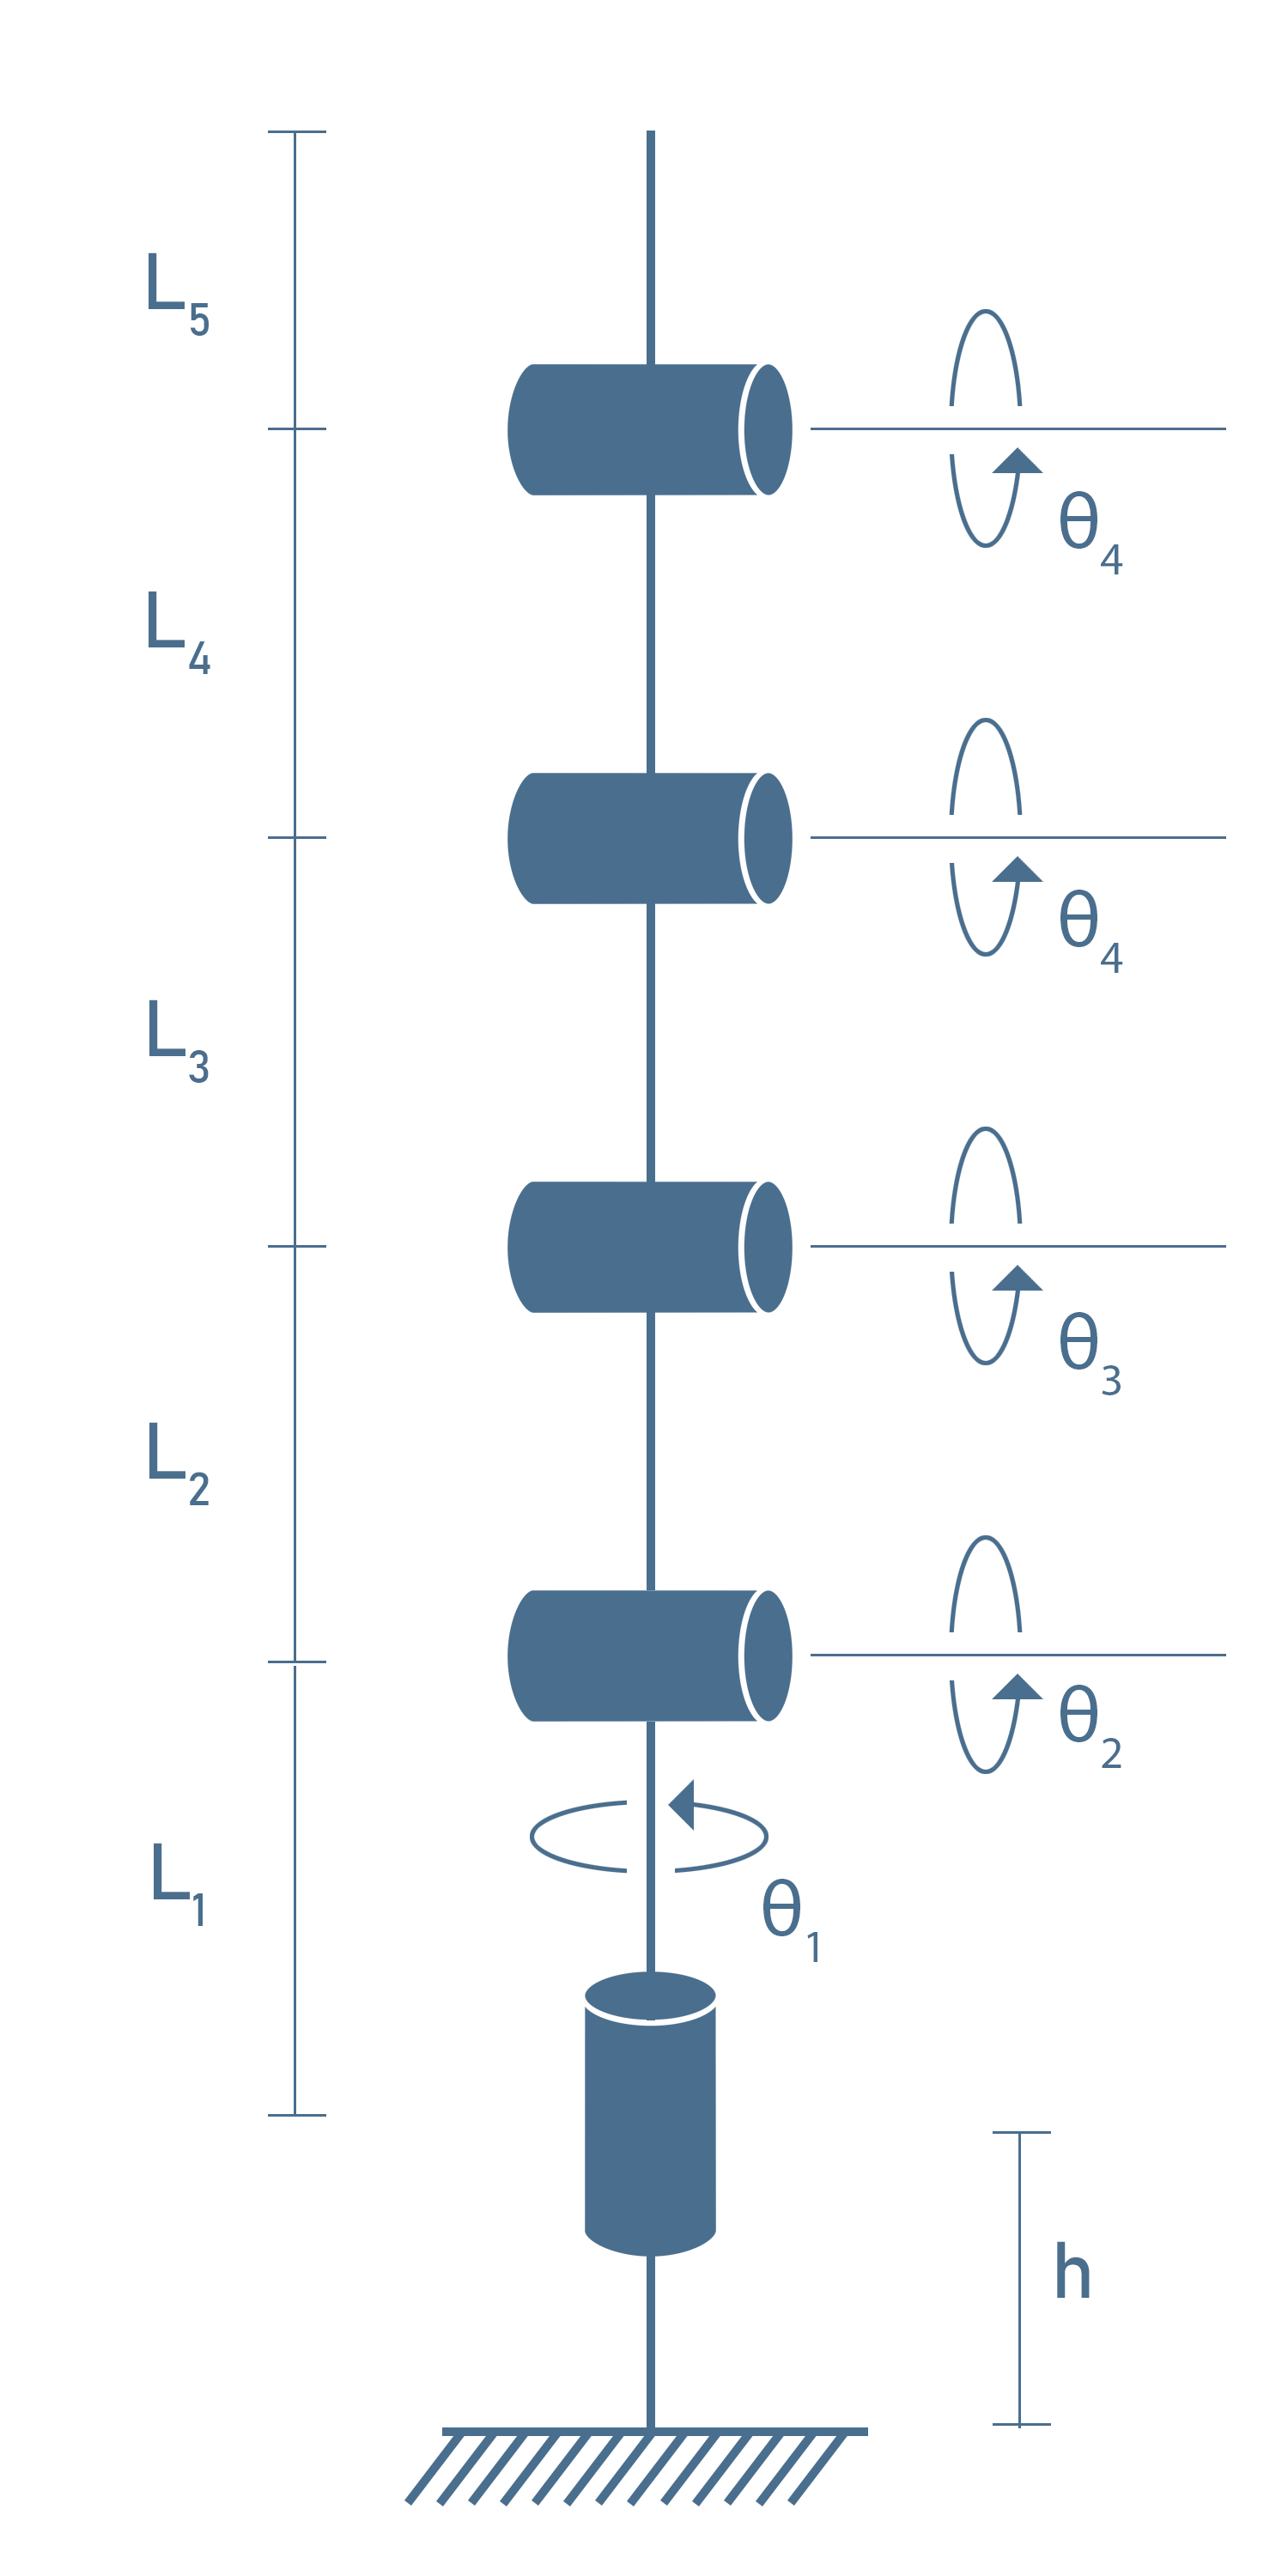
\includegraphics[width=0.3\linewidth]{../Diagrams/Model.png}
		\caption{Geometric representation}
		\label{fig:geometric}
	\end{figure}
	
	\begin{align*}
\theta_1 &= 2\mathrm{atan}\left(\frac{p_x \pm \sqrt{-d_2^2 + p_x^2 +p_y^2}}{d_2 - p_y}\right). \\[10pt]
\theta_2 &= 2\,\mathrm{atan}\left(\frac{a_z \pm \sqrt{a_x^2c_{\theta_1}^2+2a_xa_yc_{\theta_1}s_{\theta_1}+a_y^2s_{\theta_1}^2+a_z^2}}{a_xc_{\theta_1} + a_ys_{\theta_1}}\right) \\[10pt]
\theta_3 &= 
\begin{cases}
-2\,\mathrm{atan}\left(\frac{\sqrt{a_x^2c_{\theta_1}^2 + s_{2\theta_1}a_xa_y-a_y^2c_{\theta_1}^2 + a_y^2 + a_z^2} - a_zc_{\theta_2}+a_xc_{\theta_1}s_{\theta_2}+a_ys_{\theta_1}s_{\theta_2}}{a_zs_{\theta_2} + a_xc_{\theta_1}c_{\theta_2} + a_yc_{\theta_2}s_{\theta_1}}\right) \\[10pt]
2\,\mathrm{atan}\left(\frac{\sqrt{a_x^2c_{\theta_1}^2 + s_{2\theta_1}a_xa_y-a_y^2c_{\theta_1}^2 + a_y^2 + a_z^2} + a_zc_{\theta_2} - a_xc_{\theta_1}s_{\theta_2} - a_ys_{\theta_1}s_{\theta_2}}{a_zs_{\theta_2} + a_xc_{\theta_1}c_{\theta_2} + a_yc_{\theta_2}s_{\theta_1}}\right)
\end{cases} \\[10pt]
\theta_4 &= \begin{cases}
-\theta_2 - \theta_3 - \mathrm{asin}\left(\frac{d_1 - p_z + a_6n_z + a_4s_{\theta_{23}} + a_3s_{\theta_2}}{a_5}\right) \\[5pt]
\pi -\theta_2 - \theta_3 - \mathrm{asin}\left(\frac{d_1 - p_z + a_6n_z + a_4s_{\theta_{23}} + a_3s_{\theta_2}}{a_5}\right).
\end{cases} \\[10pt]
\theta_5 &= 
\begin{cases}
-\theta_3 - \theta_4 - \mathrm{asin}(n_xc_{\theta_1}s_{\theta_2} - n_zc_{\theta_2} + n_ys_{\theta_1}s_{\theta_2}) \\[5pt]
\pi - \theta_4 - \theta_3 - \mathrm{asin}(n_xc_{\theta_1}s_{\theta_2} - n_zc_{\theta_2} + n_ys_{\theta_1}s_{\theta_2}).
\end{cases}
\end{align*}

We spent quite some time trying to implement these equations to control the model in Gazebo, but unfortunately we did not get it to work. This lead to looking into ROS packages that could solve it for us. After failing to integrate both MoveIt! and  IKFast, we decided to go for another solution. Robotics System Toolbox, a add-on for MATLAB, can solve the inverse kinematics when given a URDF file, so we decided to create a MATLAB node which solved the inverse kinematics. The downside with this approach is that is a numerical solver, meaning it is quite slow.

	\subsection{D-H parameters}
	To get a model with the same link- and joint parameters as the physical robot, we measured the robot and made a new URDF model. The final model can be seen in figure \ref{fig:urdf-final}, whilst the D-H parameters can be seen in table \ref{DH-table}.
	
	\begin{figure}[H]
		\centering
		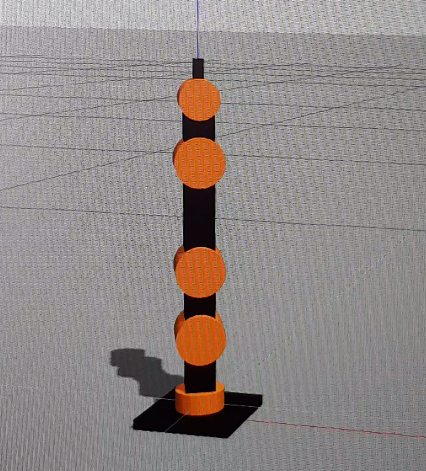
\includegraphics[width=0.7\linewidth]{../Diagrams/URDF-final.png}
		
		\caption{Final model}
		\label{fig:urdf-final}
	\end{figure}	
		
	\begin{center}           
    \begin{longtable}{| c | c | c | c | c |}
              \hline
                       
\multicolumn{5}{|c|}{\textbf{D-H parameters}} \\ \hline \endhead
\textit{Link} & \textbf{$a$} & \textbf{$\alpha$} & $d$ & \textbf{$\theta$} \\ \hline             
               1 & 0 & 0 &  0 & $\theta_1$ \\ \hline
               2 & 0 & 90 & 3 cm & $\theta_2$ \\ \hline
               3 & 7.5 cm & 0 & 0 & $\theta_3$ \\ \hline
               4 & 11.5 cm & 0 & 0 & $\theta_4$ \\ \hline
               5 & 7.3 cm & 0 & 0 & $\theta_5$ \\ \hline
               6 & 2.5 cm & 0 & 0 & 0 \\ \hline
               
\caption{D-H table}
\label{DH-table}                                       
\end{longtable}
\end{center}

	\subsection{Synchronization}
	The next step to the process was to synchronize the speed of the real robot and the simulated model. In this experiment, we ran the physical robot alongside with the Gazebo model and adjusted parameters to get synchronized movement. The result of this case study was a desired 1:1 relationship between the physical robotic arm and the model in Gazebo. Figure \ref{synch} shows the setup used to compare the speed of the model and the physical robot. 
	
	\begin{figure}[H]
		\centering
		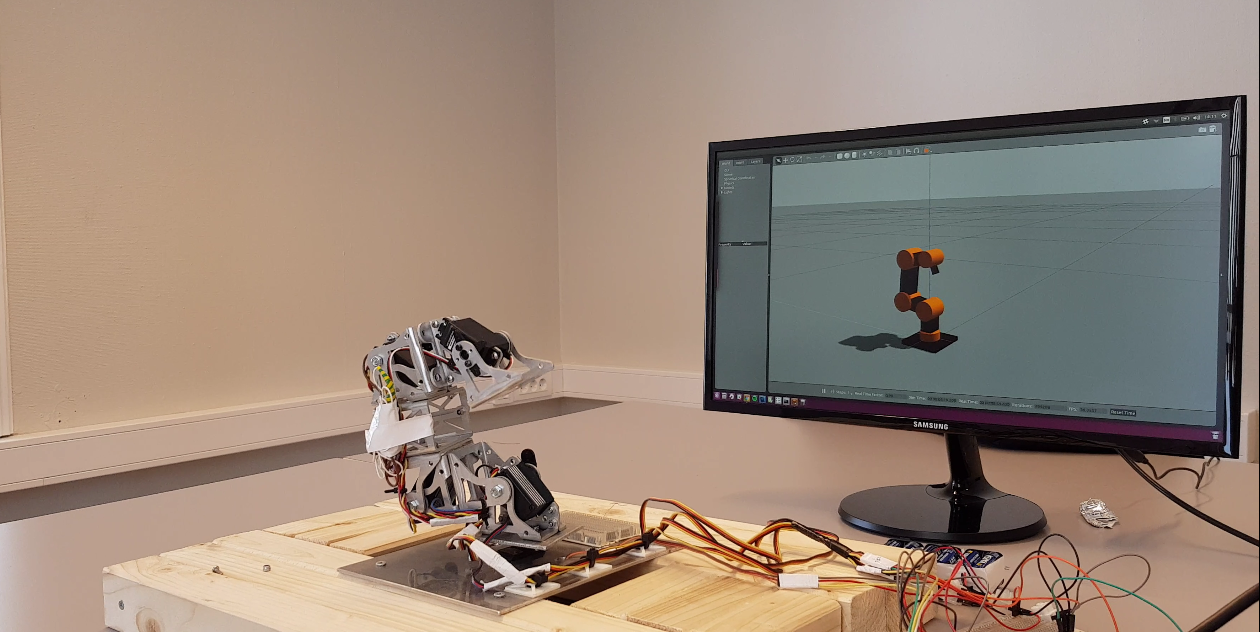
\includegraphics[width=\linewidth]{../Diagrams/Synchronizing.png}
		\caption{Synchronization}
		\label{synch}
	\end{figure}
	
	
	\subsection{Final case study}
	The final case study of ARPA included setting up the system in its entirety. The main goal was to place red markers around in the workspace of ARPA, then send a ready signal to the controller and allow ARPA move to the red marker.
	
During this final case study, the middle servo motor started operating sub-optimal. It seemed that it got weaker and could not handle the torque the way it had been doing in earlier experiments. We were still able to make ARPA touch the red marker, and were satisfied with the result of the final case study. Figure \ref{fig:three-split} shows the setup with the different views of the final case study.
	\begin{figure}[H]
		\centering
		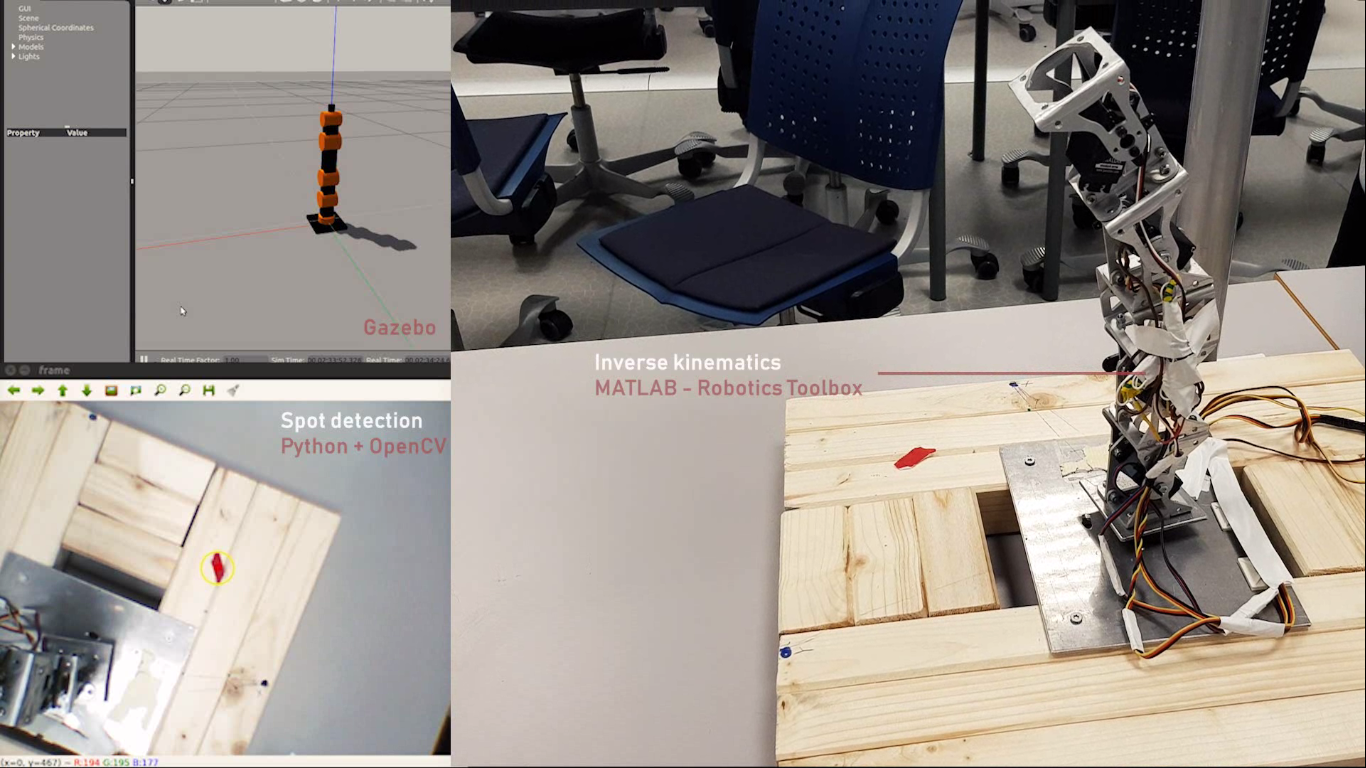
\includegraphics[width=\linewidth]{../Diagrams/ThreeSplit.png}
		\caption{Final case study}
		\label{fig:three-split}
	\end{figure}
	
	\section{Discussion}
	\label{discussion}
	Even though unexpected challenges related to the hardware arose along the project, we reached the main goals of the project and are thus satisfied with the outcome. We are pleased with the return of investment of learning ROS, and believe it will come in handy in future education and careers.
	
	
	
	\newpage



\begin{appendices}
\section{Complete kinematic solution}
\label{appendix:ik}
% the \\ insures the section title is centered below the phrase: AppendixA

\textbf{Forward kinematics:} \\

\textit{DH-parameters} are given in table \ref{tab:DH}:
\begin{table}[h!]
\centering
\begin{tabular}{| c | c | c | c | c |}
\hline
Link 		& a 			& $\alpha$ 	& d & $\theta$ \\\hline
1 & 0 		& 0 			& $d_1$ 	& $\theta_1$ \\\hline
2 & 0 		& $90^\circ$ 	& $d_2$ 	& $\theta_2$ \\\hline
3 & $a_3$ 	& 0 			& 0 		& $\theta_3$ \\\hline
4 & $a_4$ 	& 0 			& 0 		& $\theta_4$ \\\hline
5 & $a_5$ 	& 0 			& 0 		& $\theta_5$ \\\hline
6 & $a_6$ 	& 0 			& 0 		& 0 \\\hline
\end{tabular}
  \caption{This table shows some data}
  \label{tab:DH}
\end{table}

Transformation matrix $T_i^{i-1}$ is specified as:

\begin{equation*}
T_i^{i-1} = \begin{bmatrix}
c_{\theta_i} & -s_{\theta_i} & 0 & a_i \\
s_{\theta_i}c_{\alpha_i} & c_{\theta_i}c_{\alpha_i} & s_{\alpha_i} & -s_{\alpha_i}d_i \\
s_{\theta_i}s_{\alpha_i} & c_{\theta_i}s_{\alpha_i} & c_{\alpha_i} & c_{\alpha_i}d_i \\
0 & 0 & 0 & 1
\end{bmatrix}
\end{equation*}

With the input of the DH-parameters, the following matrices are derived:

\begin{equation*}
\begin{split}
A_{1} =
&\begin{bmatrix}
c_{\theta_1} & -s_{\theta_1} & 0 & 0 \\
s_{\theta_1} & c_{\theta_1} & 0 & 0 \\
0 & 0 & 1 & d_1 \\
0 & 0 & 0 & 1			 
\end{bmatrix},\,
A_{2} =
\begin{bmatrix}
c_{\theta_2} & -s_{\theta_2} & 0 & 0 \\
0 & 0 & -1 & -d_2 \\
s_{\theta_2} & c_{\theta_2} & 0 & 0 \\
0 & 0 & 0 & 1			 
\end{bmatrix} \\\\
A_{3} =
&\begin{bmatrix}
c_{\theta_3} & -s_{\theta_3} & 0 & a_3 \\
s_{\theta_3} & c_{\theta_3} & 0 & 0 \\
0 & 0 & 1 & 0 \\
0 & 0 & 0 & 1			 
\end{bmatrix},\,
A_{4} =
\begin{bmatrix}
c_{\theta_4} & -s_{\theta_4} & 0 & a_4 \\
s_{\theta_4} & c_{\theta_4} & 0 & 0 \\
0 & 0 & 1 & 0 \\
0 & 0 & 0 & 1			 
\end{bmatrix} \\\\
A_{5} =
&\begin{bmatrix}
c_{\theta_5} & -s_{\theta_5} & 0 & a_5 \\
s_{\theta_5} & c_{\theta_5} & 0 &0 \\
0 & 0 & 1 & 0 \\
0 & 0 & 0 & 1			 
\end{bmatrix},\,
A_{6} =
\begin{bmatrix}
1 & 0 & 0 & a_6 \\
0 & 1 & 0 & 0 \\
0 & 0 & 1 & 0 \\
0 & 0 & 0 & 1			 
\end{bmatrix}
\end{split}
\end{equation*}
\newpage
$T_0^6$ gives a set of linear equations for forward kinematics:

\begin{equation*}
\begin{split}
&T_{H}^{R} = T_{0}^{6} =
\begin{bmatrix}
n_x & o_x & a_x & p_x \\
n_y & o_y & a_y & p_y \\
n_z & o_z & a_z & p_z \\
0 & 0 & 0 & 1			 
\end{bmatrix}
= A_1 A_2 A_3 A_4 A_5 A_6 \\\\
=\, &\begin{bmatrix}
c_{\theta_{2345}}c_{\theta_1} & -s_{\theta_{2345}}c_{\theta_1} & s_{\theta_1} & d_2s_{\theta_1} + a_6c_{\theta_{2345}}c_{\theta1} + a_4c_{\theta_{23}}c_{\theta_1} + a_3c_{\theta_1}c_{\theta_2} + a_5c_{\theta_{234}}c_{\theta_1} \\
c_{\theta_{2345}}s_{\theta1} & 
-s_{\theta_{2345}}s_{\theta_1} & 
-c_{\theta_1} & 
a_6c_{\theta_{2345}}s_{\theta_1} - d_2c_{\theta1} + a_4c_{\theta_{23}}s_{\theta_1} + a_3c_{\theta_2}s_{\theta1} + a_5c_{\theta_{234}}s_{\theta_1} \\
s_{\theta_{2345}} & c_{\theta_{2345}} & 0 & d_1 + a_6s_{\theta_{2345}} + a_4s_{\theta_{23}} + a_3s_{\theta_2} + a_5s_{\theta_{234}} \\
0 & 0 & 0 & 1			 
\end{bmatrix} \\\\
\end{split}
\end{equation*}
\newpage
\noindent\textbf{Inverse kinematics:} \\
The full set of equations for the inverse kinematics are summarized at the end of this section.
\begin{align*}
\begin{split}
&(T_{1}^{0})^{-1}T_{6}^{0} =
T_{2}^{1}T_{3}^{2}T_{4}^{3}T_{5}^{4}T_{6}^{5} \\\\
\Rightarrow\, &A_{1}^{-1} \times
\begin{bmatrix}
n_x & o_x & a_x & p_x \\
n_y & o_y & a_y & p_y \\
n_z & o_z & a_z & p_z \\
0 & 0 & 0 & 1	
\end{bmatrix} = A_2 A_3 A_4 A_5 A_6 \\\\
\Rightarrow\, &\begin{bmatrix}
c_{\theta_1} & s_{\theta_1} & 0 & 0 \\
-s_{\theta_1} & c_{\theta_1} & 0 & 0 \\
0 & 0 & 1 & -d_1 \\
0 & 0 & 0 & 1	
\end{bmatrix} \times 
\begin{bmatrix}
n_x & o_x & a_x & p_x \\
n_y & o_y & a_y & p_y \\
n_z & o_z & a_z & p_z \\
0 & 0 & 0 & 1	
\end{bmatrix} = 
A_2 A_3 A_4 A_5 A_6 \\\\
\Rightarrow\,
&\begin{bmatrix}
n_xc_{\theta_1} + n_ys_{\theta_1} & o_xc_{\theta_1} + o_ys_{\theta_1} & a_xc_{\theta_1} + a_ys_{\theta_1} & p_xc_{\theta_1} + p_ys_{\theta_1} \\
n_yc_{\theta_1} - n_xs_{\theta_1} & o_yc_{\theta_1} - o_xs_{\theta_1} & a_yc_{\theta_1} - a_xs_{\theta_1} & p_yc_{\theta_1} - p_xs_{\theta_1} \\
n_z & o_z & a_z & p_z - d_1 \\
0 & 0 & 0 & 1	
\end{bmatrix} \\\\ =\,
&\begin{bmatrix}
c_{\theta_{2345}} & -s_{\theta_{2345}} & 0 & a_6c_{\theta_{2345}} + a_4c_{\theta_{23}} + a_3c_{\theta_2} + a_5c_{\theta_{234}} \\
0 & 0 & -1 & -d_2 \\
s_{\theta_{2345}} & c_{\theta_{2345}} & 0 & a_6s_{\theta_{2345}} + a_4s_{\theta_{23}} + a_3s_{\theta_2} + a_5s_{\theta_{234}} \\
0 & 0 & 0 & 1
\end{bmatrix}
\end{split}
\end{align*}
Equating elements at \textit{(2, 4)} to find $\theta_1$, and elements at \textit{(3, 4)} to find $\theta_4$: \\
\begin{equation}
\begin{split}
&p_yc_{\theta_1} - p_xs_{\theta_1} = -d_2 \\
\Rightarrow\,
&\theta_1 = 2\mathrm{atan}\left(\frac{p_x \pm \sqrt{-d_2^2 + p_x^2 +p_y^2}}{d_2 - p_y}\right). \\\\
\end{split}
\end{equation}
\begin{equation}
\begin{split}
&p_z - d_1 = a_6s_{\theta_{2345}} + a_4s_{\theta_{23}} + a_3s_{\theta_2} + a_5s_{\theta_{234}} \\\\
\Rightarrow\,
&p_z - d_1 = a_6n_z + a_4s_{\theta_{23}} + a_3s_{\theta_2} + a_5s_{\theta_{234}} \\\\
\Rightarrow\,
&\theta_4 = \begin{cases}
    -\theta_2 - \theta_3 - \mathrm{asin}\left(\frac{d_1 - p_z + a_6n_z + a_4s_{\theta_{23}} + a_3s_{\theta_2}}{a_5}\right) \\
    \pi -\theta_2 - \theta_3 - \mathrm{asin}\left(\frac{d_1 - p_z + a_6n_z + a_4s_{\theta_{23}} + a_3s_{\theta_2}}{a_5}\right).
  \end{cases} \\
 \end{split}
\end{equation}
\newpage
\begin{equation*}
\begin{split}
&(T_{2}^{0})^{-1}T_{6}^{0} =
T_{3}^{2}T_{4}^{3}T_{5}^{4}T_{6}^{5} \\\\
\Rightarrow \, &(A_{1}A_{2})^{-1} \times
\begin{bmatrix}
n_x & o_x & a_x & p_x \\
n_y & o_y & a_y & p_y \\
n_z & o_z & a_z & p_z \\
0 & 0 & 0 & 1	
\end{bmatrix} = A_3 A_4 A_5 A_6 \\\\
\Rightarrow\, &\begin{bmatrix}
c_{\theta_1}c_{\theta_2} & c_{\theta_2}s_{\theta_1} & s_{\theta_2} & -d_1s_{\theta_2} \\
-c_{\theta_1}s_{\theta_2} & -s_{\theta_1}s_{\theta_2} & c_{\theta_2} & -d_1c_{\theta_2} \\
s_{\theta_1} & -c_{\theta_1} & 0 & -d_2 \\
0 & 0 & 0 & 1	
\end{bmatrix} \times 
\begin{bmatrix}
n_x & o_x & a_x & p_x \\
n_y & o_y & a_y & p_y \\
n_z & o_z & a_z & p_z \\
0 & 0 & 0 & 1	
\end{bmatrix} = 
A_3 A_4 A_5 A_6 \\\\
\Rightarrow\,
&\begin{bmatrix}
r_{11} & r_{12} & r_{13} & r_{14} \\
r_{21} & r_{22} & r_{23} & r_{24} \\
r_{31} & r_{32} & r_{33} & r_{34} \\
r_{41} & r_{42} & r_{43} & r_{44} \\
\end{bmatrix} =
\begin{bmatrix}
c_{\theta_{345}} & -s_{\theta_{345}} & 0 & a_3 + a_5c_{\theta_{34}} + a_4c_{\theta_3} + a_6c_{\theta_{345}} \\
s_{\theta_{345}} & c_{\theta_{345}} & 0 & a_5s_{\theta_{34}} + a_4s_{\theta_3} + a_6s_{\theta_{345}} \\
0 & 0 & 1 & 0 \\
0 & 0 & 0 & 1
\end{bmatrix}
\end{split}
\end{equation*}
where: \\
\begin{align*}
\begin{split}
r_{11} &= n_zs_{\theta_2} + n_xc_{\theta_1}c_{\theta_2} + n_yc_{\theta_2}s_{\theta_1} \\
r_{12} &= o_zs_{\theta_2} + o_xc_{\theta_1}c_{\theta_2} + o_yc_{\theta_2}s_{\theta_1} \\
r_{13} &= a_zs_{\theta_2} + a_xc_{\theta_1}c_{\theta_2} + a_yc_{\theta_2}s_{\theta_1} \\
r_{14} &= p_zs_{\theta_2} - d_1s_{\theta_2} + p_xc_{\theta_1}c_{\theta_2} + p_yc_{\theta_2}s_{\theta_1}\\
r_{21} &= n_zc_{\theta_2} - n_xc_{\theta_1}s_{\theta_2} - n_ys_{\theta_1}s_{\theta_2}\\
r_{22} &= o_zc_{\theta_2} - o_xc_{\theta_1}s_{\theta_2} - o_ys_{\theta_1}s_{\theta_2} \\
r_{23} &= a_zc_{\theta_2} - a_xc_{\theta_1}s_{\theta_2} - a_ys_{\theta_1}s_{\theta_2}\\
r_{24} &= p_zc_{\theta_2} - d_1c_{\theta_2} - p_xc_{\theta_1}s_{\theta_2} - p_ys_{\theta_1}s_{\theta_2}\\
r_{31} &= n_xs_{\theta_1} - n_yc_{\theta_1}\\
r_{32} &= o_xs_{\theta_1} - o_yc_{\theta_1}\\
r_{33} &= a_xs_{\theta_1} - a_yc_{\theta_1}\\
r_{34} &= p_xs_{\theta_1} - p_yc_{\theta_1} - d_2\\
r_{41} &= 0\\
r_{42} &= 0\\
r_{43} &= 0\\
r_{44} &= 1\\
\end{split}
\end{align*}
\newpage
Equating elements at \textit{(1, 3)} to find $\theta_2$ and \textit{(2, 1)} to find $\theta_5$: \\
\begin{align*}
&a_zs_{\theta_2} + a_xc_{\theta_1}c_{\theta_2} + a_yc_{\theta_2}s_{\theta_1} = 0 \\[10pt]
\Rightarrow\, &\theta_2 = 2\,\mathrm{atan}\left(\frac{a_z \pm \sqrt{a_x^2c_{\theta_1}^2+2a_xa_yc_{\theta_1}s_{\theta_1}+a_y^2s_{\theta_1}^2+a_z^2}}{a_xc_{\theta_1} + a_ys_{\theta_1}}\right). \\[10pt]
&n_zc_{\theta_2} - n_xc_{\theta_1}s_{\theta_2} - n_ys_{\theta_1}s_{\theta_2} = s_{\theta_{345}} \\[10pt]
\Rightarrow\, &\theta_5 = 
\begin{cases}
-\theta_3 - \theta_4 - \mathrm{asin}(n_xc_{\theta_1}s_{\theta_2} - n_zc_{\theta_2} + n_ys_{\theta_1}s_{\theta_2}) \\[5pt]
\pi - \theta_4 - \theta_3 - \mathrm{asin}(n_xc_{\theta_1}s_{\theta_2} - n_zc_{\theta_2} + n_ys_{\theta_1}s_{\theta_2}).
\end{cases} \\
\end{align*}
\newpage
\begin{equation*}
\begin{split}
&(T_{3}^{0})^{-1}T_{6}^{0} =
T_{4}^{3}T_{5}^{4}T_{6}^{5} \\\\
\Rightarrow \, &(A_{1}A_{2}A_{3})^{-1} \times
\begin{bmatrix}
n_x & o_x & a_x & p_x \\
n_y & o_y & a_y & p_y \\
n_z & o_z & a_z & p_z \\
0 & 0 & 0 & 1	
\end{bmatrix} = A_4 A_5 A_6 \\\\
\Rightarrow\, &\begin{bmatrix}
c_{\theta_{23}}c_{\theta_1} & c_{\theta_{23}}s_{\theta_1} & s_{\theta_{23}} & -d_1s_{\theta_{23}} - a_3c_{\theta_3} \\
-s_{\theta_{23}}c_{\theta_1} & -s_{\theta_{23}}s_{\theta_1} & c_{\theta_{23}} & a_3s_{\theta_3} - d_1c_{\theta_{23}} \\
s_{\theta_1} & -c_{\theta_1} & 0 & -d_2 \\
0 & 0 & 0 & 1
\end{bmatrix} \times 
\begin{bmatrix}
n_x & o_x & a_x & p_x \\
n_y & o_y & a_y & p_y \\
n_z & o_z & a_z & p_z \\
0 & 0 & 0 & 1	
\end{bmatrix} = 
A_4 A_5 A_6 \\\\
\Rightarrow\,
&\begin{bmatrix}
r_{11} & r_{12} & r_{13} & r_{14} \\
r_{21} & r_{22} & r_{23} & r_{24} \\
r_{31} & r_{32} & r_{33} & r_{34} \\
r_{41} & r_{42} & r_{43} & r_{44} \\
\end{bmatrix} =
\begin{bmatrix}
c_{\theta_{45}} & -s_{\theta_{45}} & 0 & a_4 + a_6c_{\theta_{45}} + a_5c_{\theta_4} \\
s_{\theta_{45}} & c_{\theta_{45}} & 0 & a_6s_{\theta_{45}} + a_5s_{\theta_4} \\
0 & 0 & 1 & 0 \\
0 & 0 & 0 & 1
\end{bmatrix}\\
\end{split}
\end{equation*}
where: \\
\begin{align*}
\begin{split}
r_{13} &= a_zc_{\theta_2}s_{\theta_3} + a_zc_{\theta_3}s_{\theta_2} + a_xc_{\theta_1}c_{\theta_2}c_{\theta_3} + a_yc_{\theta_2}c_{\theta_3}s_{\theta_1} - a_xc_{\theta_1}s_{\theta_2}s_{\theta_3} - a_ys_{\theta_1}s_{\theta_2}s_{\theta_3} \\
& = a_z(c_{\theta_2}s_{\theta_3} + c_{\theta_3}s_{\theta_2}) + c_{\theta_2}c_{\theta_3}(a_xc_{\theta_1} + a_ys_{\theta_1}) -s_{\theta_2}s_{\theta_3}(a_xc_{\theta_1} + a_ys_{\theta_1})
\end{split}
\end{align*}
Equating elements at \textit{(1, 3)} to find $\theta_3$: \\
\begin{align*}
\Rightarrow\, &\theta_3 = 
\begin{cases}
-2\,\mathrm{atan}\left(\frac{\sqrt{a_x^2c_{\theta_1}^2 + s_{2\theta_1}a_xa_y-a_y^2c_{\theta_1}^2 + a_y^2 + a_z^2} - a_zc_{\theta_2}+a_xc_{\theta_1}s_{\theta_2}+a_ys_{\theta_1}s_{\theta_2}}{a_zs_{\theta_2} + a_xc_{\theta_1}c_{\theta_2} + a_yc_{\theta_2}s_{\theta_1}}\right) \\[10pt]
2\,\mathrm{atan}\left(\frac{\sqrt{a_x^2c_{\theta_1}^2 + s_{2\theta_1}a_xa_y-a_y^2c_{\theta_1}^2 + a_y^2 + a_z^2} + a_zc_{\theta_2} - a_xc_{\theta_1}s_{\theta_2} - a_ys_{\theta_1}s_{\theta_2}}{a_zs_{\theta_2} + a_xc_{\theta_1}c_{\theta_2} + a_yc_{\theta_2}s_{\theta_1}}\right)
\end{cases} \\
\end{align*}
\newpage
Angles $\theta_1,\,\theta_2,\,\theta_3,\,\theta_4,\,\theta_5$ are given by the following equations: \\
\begin{align*}
\theta_1 &= 2\mathrm{atan}\left(\frac{p_x \pm \sqrt{-d_2^2 + p_x^2 +p_y^2}}{d_2 - p_y}\right). \\[10pt]
\theta_2 &= 2\,\mathrm{atan}\left(\frac{a_z \pm \sqrt{a_x^2c_{\theta_1}^2+2a_xa_yc_{\theta_1}s_{\theta_1}+a_y^2s_{\theta_1}^2+a_z^2}}{a_xc_{\theta_1} + a_ys_{\theta_1}}\right) \\[10pt]
\theta_3 &= 
\begin{cases}
-2\,\mathrm{atan}\left(\frac{\sqrt{a_x^2c_{\theta_1}^2 + s_{2\theta_1}a_xa_y-a_y^2c_{\theta_1}^2 + a_y^2 + a_z^2} - a_zc_{\theta_2}+a_xc_{\theta_1}s_{\theta_2}+a_ys_{\theta_1}s_{\theta_2}}{a_zs_{\theta_2} + a_xc_{\theta_1}c_{\theta_2} + a_yc_{\theta_2}s_{\theta_1}}\right) \\[10pt]
2\,\mathrm{atan}\left(\frac{\sqrt{a_x^2c_{\theta_1}^2 + s_{2\theta_1}a_xa_y-a_y^2c_{\theta_1}^2 + a_y^2 + a_z^2} + a_zc_{\theta_2} - a_xc_{\theta_1}s_{\theta_2} - a_ys_{\theta_1}s_{\theta_2}}{a_zs_{\theta_2} + a_xc_{\theta_1}c_{\theta_2} + a_yc_{\theta_2}s_{\theta_1}}\right)
\end{cases} \\[10pt]
\theta_4 &= \begin{cases}
-\theta_2 - \theta_3 - \mathrm{asin}\left(\frac{d_1 - p_z + a_6n_z + a_4s_{\theta_{23}} + a_3s_{\theta_2}}{a_5}\right) \\[5pt]
\pi -\theta_2 - \theta_3 - \mathrm{asin}\left(\frac{d_1 - p_z + a_6n_z + a_4s_{\theta_{23}} + a_3s_{\theta_2}}{a_5}\right).
\end{cases} \\[10pt]
\theta_5 &= 
\begin{cases}
-\theta_3 - \theta_4 - \mathrm{asin}(n_xc_{\theta_1}s_{\theta_2} - n_zc_{\theta_2} + n_ys_{\theta_1}s_{\theta_2}) \\[5pt]
\pi - \theta_4 - \theta_3 - \mathrm{asin}(n_xc_{\theta_1}s_{\theta_2} - n_zc_{\theta_2} + n_ys_{\theta_1}s_{\theta_2}).
\end{cases}
\end{align*}

\section{GitHub repository}
Link to GitHub: https://github.com/andrehaland/DFSM3200-robotic-arm

\end{appendices}

\newpage
	
	
\begin{thebibliography}{1}

\bibitem{berge2015} Aslak Berge. Avhengig av polske kniver. \textit{http://ilaks.no/avhengig-av-polske-kniver-2/}. Aug 2018.

\bibitem{digre2014} Hanne Digre. Lønnsom foredling av sjømat i Norge. 2014.

\bibitem{baba2017} Abdellatif Baba.Robot arm control with Arduino. June 2017.

\bibitem{walker2012} Jeffry Walker, Joshua Beverly, Christopher Cook, Migueal de Rojas. Anthropomorphic Robotic Manipulator (ARM). 2012

\bibitem{turtle2017} Open Source Robotics Foundation. Understanding ROS Nodes.
\textit{http://wiki.ros.org/ROS/Tutorials/UnderstandingNodes}. Aug 2017.

\bibitem{arduino} Arduino. Arduino libraries. \textit{https://www.arduino.cc/en/Reference/Libraries}

\bibitem{joseph2015} Lentin Joseph. Mastering ROS for Robotics Programming. Des 2015



\newpage	

\end{thebibliography}	
	

\end{document}
